% Mini research note for sharpness and robustness-aware Raman suppression.
\documentclass[11pt]{article}
% Shared preamble for the research-note series.
% Create note-specific content in the per-note directory; keep common macros here.
\usepackage[margin=1in]{geometry}
\usepackage[T1]{fontenc}
\usepackage[utf8]{inputenc}
\usepackage{amsmath,amssymb}
\usepackage{booktabs,longtable,array}
\usepackage{graphicx}
\usepackage{float}
\usepackage{enumitem}
\usepackage{xcolor}
\usepackage{hyperref}
\usepackage{caption}
\usepackage{titlesec}
\hypersetup{colorlinks=true, linkcolor=blue!60!black, urlcolor=blue!60!black, citecolor=blue!60!black}
\setlist[itemize]{leftmargin=1.25em, itemsep=0.2em, topsep=0.3em}
\setlist[enumerate]{leftmargin=1.4em, itemsep=0.2em, topsep=0.3em}
\setlength{\parindent}{0pt}
\setlength{\parskip}{0.6em}
\newcommand{\statusbox}[2]{%
  \noindent\fcolorbox{black}{gray!10}{%
    \parbox{\dimexpr\linewidth-2\fboxsep-2\fboxrule\relax}{%
      \textbf{Status:} #1\\#2
    }%
  }
}

% Shared notation helpers for the research-note series.
\newcommand{\Jlin}{J}
\newcommand{\Jphys}{J_{\mathrm{phys}}}
\newcommand{\Jsurf}{J_{\mathrm{surf}}}
\newcommand{\JdB}{J_{\mathrm{dB}}}
\newcommand{\phiopt}{\phi_{\mathrm{opt}}}
\newcommand{\sigmathreedb}{\sigma_{3\mathrm{dB}}}
\newcommand{\Nt}{N_t}
\newcommand{\Nphi}{N_{\phi}}
\newcommand{\Lfiber}{L}
\newcommand{\Pcont}{P}
\newcommand{\band}{\mathcal{B}_{\mathrm{Raman}}}
\newcommand{\todoitem}[1]{\textcolor{red!70!black}{\textbf{TODO:} #1}}


\title{Sharpness, Robustness Penalties, and Hessian Geometry}
\author{Fiber Raman Suppression Project}
\date{Evidence snapshot: 2026-04-26}

\begin{document}
\maketitle

\begin{abstract}
This note asks whether the default Raman-suppression optimizer should be
replaced by an explicitly robustness-aware objective. The tested alternatives
were Monte Carlo averaging over phase perturbations, sharpness-aware
minimization, and a finite-difference Hessian-trace penalty. The main result is
negative but useful: the plain log-cost optimizer remains the best default when
the goal is maximum Raman suppression, while Monte Carlo and trace penalties
are optional tools when tolerance to phase-shaper error matters more than
depth. The geometry result is also important: every resolved Hessian spectrum
in this sweep stayed indefinite, so these solutions are better understood as
saddle-like stationary points rather than clean convex minima.
\end{abstract}

\section*{Claim Status}
\statusbox{established tradeoff; not a default replacement}{The sweep supports
a stable conclusion: robustness penalties can buy perturbation tolerance, but
they cost Raman depth and do not remove saddle-like curvature. The plain
objective remains the default. The robustness objectives are useful research
knobs, not a new universal optimizer.}

\section{Question and Thesis}

The baseline note defines the usual objective: choose a spectral phase
\(\phi(\omega)\), propagate the pulse through the fiber, and minimize the
Raman-band output fraction. This note asks a different question:

\[
    \text{Can we optimize not only for a deep result, but for a less fragile
    result?}
\]

The motivation is practical. A phase mask that gives excellent suppression in
simulation may be hard to use experimentally if small phase errors ruin it. A
more robust mask might tolerate small shaper errors, calibration drift, or
minor parameter mismatch. In this project, robustness is measured by how large
a random phase perturbation can be before the solution loses \(3\,\mathrm{dB}\)
of suppression.

The thesis is:
\[
    \text{robustness can be improved, but it is not free.}
\]
The strongest trace-penalty results widen the perturbation tolerance, but they
also give much shallower Raman suppression. Monte Carlo averaging gives a
smaller but cheaper tolerance improvement. Sharpness-aware minimization did not
produce a useful Pareto improvement in this sweep. None of the variants turned
the local Hessian into a positive-definite minimum.

\subsection*{Intuition Check}

The plain optimizer asks, ``how low can the Raman objective go?'' The robust
objectives ask, ``can the result stay good if the phase is nudged?'' These are
not the same question. A very deep optimum can be narrow and fragile, while a
shallower optimum can be wider and easier to tolerate.

\section{Common Setup}

All results in this note use the same phase-only control idea as the baseline:
\[
    u_\omega(0;\phi)=u_{\omega,0}\exp(i\phi(\omega)).
\]
The output Raman objective is the Raman-band energy fraction
\[
    \Jphys(\phi)
    =
    \frac{
    \sum_{\omega_k\in\band}|u_{\omega_k}(L;\phi)|^2\,\Delta\omega
    }{
    \sum_k |u_{\omega_k}(L;\phi)|^2\,\Delta\omega
    },
\]
reported in decibels as
\[
    \JdB(\phi)=10\log_{10}\Jphys(\phi).
\]
Lower \(\JdB\) is deeper suppression. The forward propagation follows the
standard GNLSE modeling stack for nonlinear fiber optics
\cite{agrawal2019,dudley2006,hult2007}. L-BFGS is used for the first-order
optimization step \cite{liu1989,nocedal2006}.

Two operating points were used. The first is a full-grid SMF-28 point at
\(L=0.5\,\mathrm{m}\), \(P=0.05\,\mathrm{W}\), and \(\Nt=8192\). The second is
a reduced-control SMF-28 point with \(57\) cubic-basis coefficients. The
reduced-control point is included because a robustness method should be tested
both on the direct full-grid parameterization and on a structured control
space.

\begin{figure}[H]
\centering
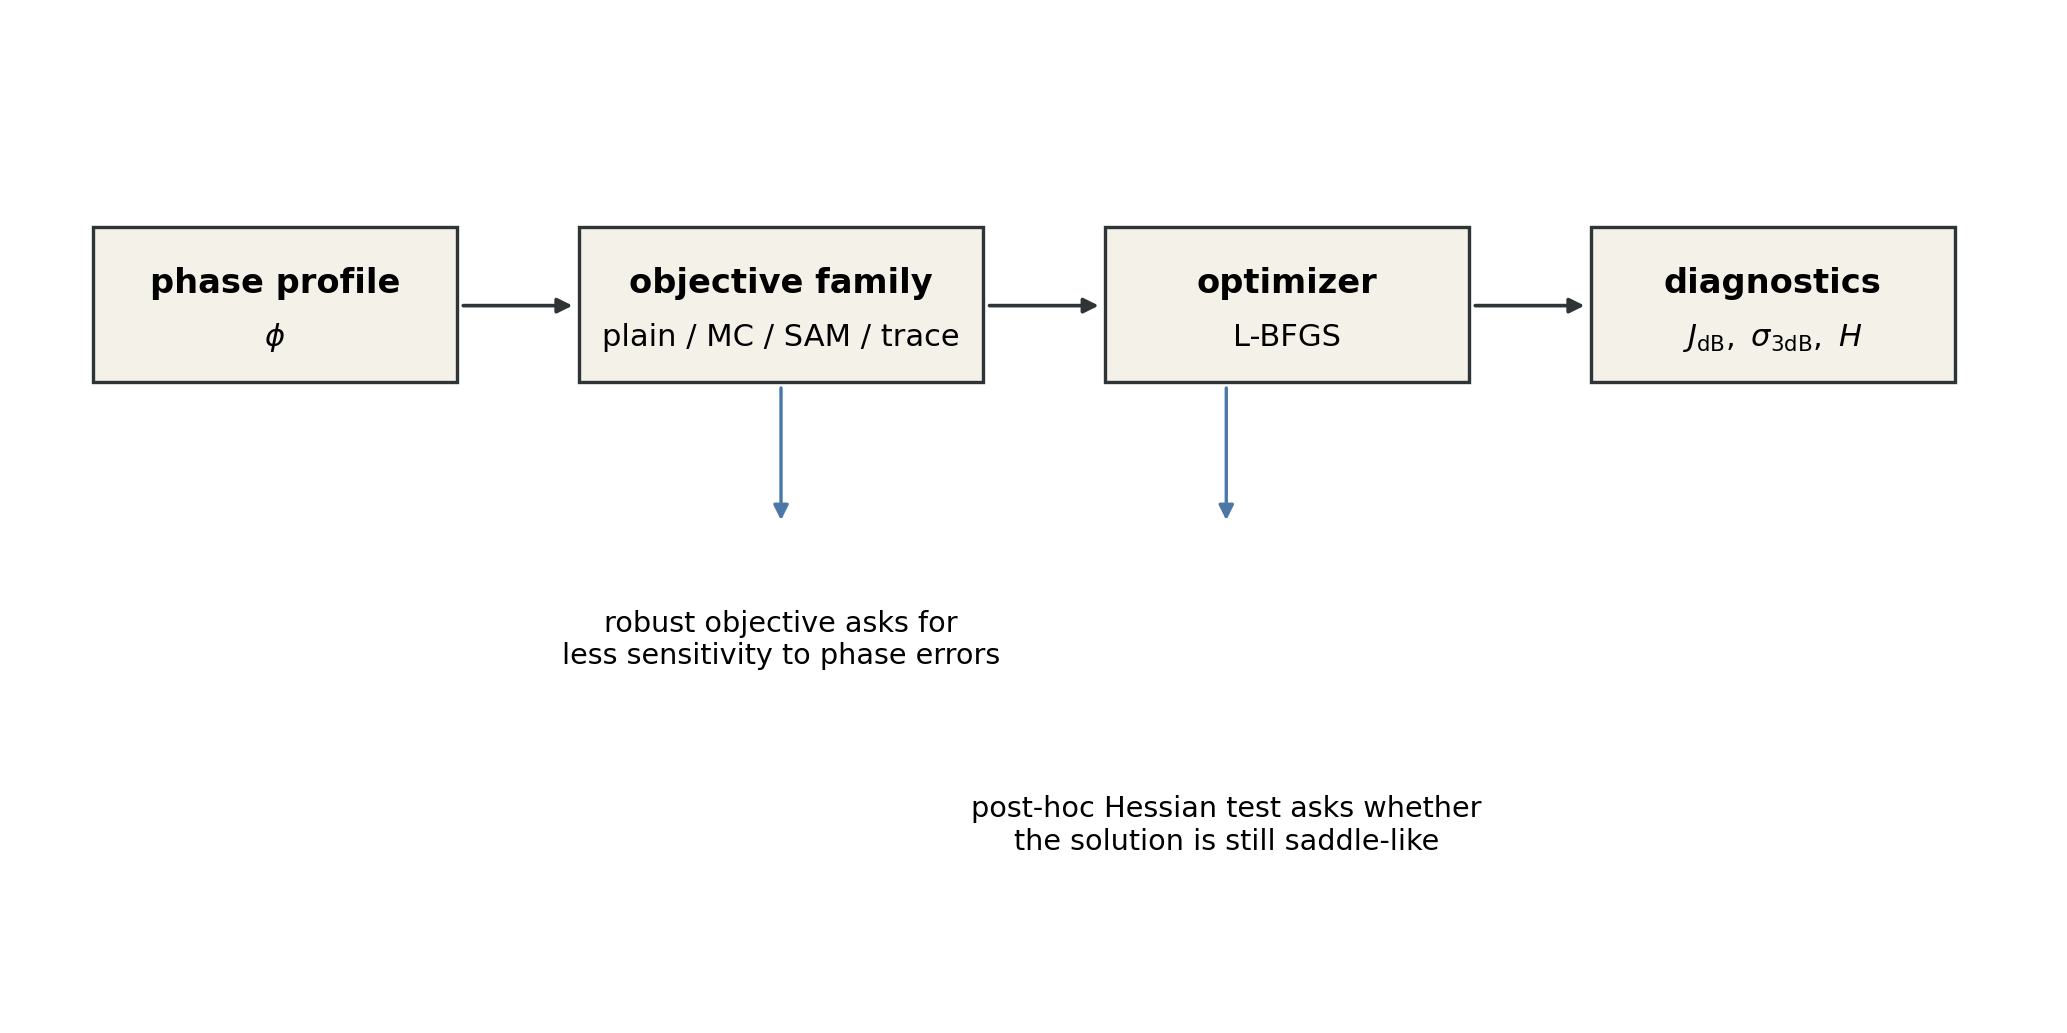
\includegraphics[width=0.94\linewidth]{figures/sharpness_workflow_diagram.png}
\caption{Sharpness/robustness workflow. The physical propagation model is the
same as the baseline. This research lane changes the objective family and then
diagnoses the resulting solution with suppression depth, perturbation
tolerance, and Hessian curvature.}
\end{figure}

\section{Robust Objective Variants}

Let \(F(\phi)\) denote the log-scale Raman objective optimized by L-BFGS. The
plain baseline solves
\[
    \min_\phi F(\phi).
\]
The robustness variants modify the scalar objective before L-BFGS sees it.

\subsection{Monte Carlo Phase Averaging}

The Monte Carlo objective minimizes expected performance under random phase
error:
\[
    F_{\mathrm{MC}}(\phi)
    =
    \frac{1}{K}
    \sum_{k=1}^{K}
    F(\phi+\epsilon_k),
    \qquad
    \epsilon_k\sim\mathcal{N}(0,\sigma^2 I).
\]
In the implementation, the perturbation bank is fixed during one optimization
run and uses antithetic pairs \((+\epsilon,-\epsilon)\). This matters because
L-BFGS expects a deterministic objective during line search. If new random
noise were drawn every call, the optimizer would chase a moving target.

\subsection*{Intuition Check}

Monte Carlo averaging is the most literal robustness objective: instead of
grading one exact phase mask, we grade nearby masks too. If a solution only
works at one razor-thin phase setting, this averaged objective punishes it.

\subsection{Sharpness-Aware Perturbed Loss}

Sharpness-aware minimization (SAM) approximately solves a local min-max
problem:
\[
    F_{\mathrm{SAM}}(\phi)
    =
    F\!\left(\phi+\rho
    \frac{\nabla_\phi F(\phi)}{\|\nabla_\phi F(\phi)\|}
    \right).
\]
The perturbation direction is the local steepest direction in phase space, and
\(\rho\) sets the neighborhood radius. The idea comes from sharpness-aware
training in machine learning \cite{foret2021}. Related work warns that
sharpness measures can be scale-sensitive or misleading, so this note treats
SAM as one robustness probe, not as the definition of flatness
\cite{kwon2021,zhuang2022}.

\subsection*{Intuition Check}

SAM asks, ``if I step in the direction that locally makes the cost worse, is
the result still okay?'' That is a useful stress test, but it is not identical
to real shaper noise, and it does not guarantee that the Hessian is flat.

\subsection{Hessian-Trace Penalty}

The trace-penalty objective adds a finite-difference estimate of local
curvature:
\[
    F_{\mathrm{trace}}(\phi)
    =
    F(\phi) + \lambda_{\mathrm{tr}} S(\phi),
\]
where
\[
    S(\phi)
    \approx
    \frac{1}{N_s}
    \sum_{i=1}^{N_s}
    \frac{
    F(\phi+\epsilon Pv_i)
    +F(\phi-\epsilon Pv_i)
    -2F(\phi)
    }{\epsilon^2}.
\]
Here \(v_i\) are fixed Rademacher probe vectors, and \(P\) projects out two
gauge directions: constant phase and linear phase over the input band. Those
directions do not represent meaningful Raman-control changes, so the sharpness
estimator should not spend probes measuring them. Hutchinson-style trace
estimation is a standard way to estimate matrix traces without forming the
matrix explicitly \cite{hutchinson1989,meyer2021}.

\subsection*{Intuition Check}

The trace penalty is trying to punish directions where the objective bends
sharply. But the Raman landscape is not a simple bowl. It has both upward and
downward curvature directions, so a signed trace can hide cancellation. That
is why the note also checks Hessian eigenvalues after optimization.

\section{Robustness and Hessian Diagnostics}

The main robustness metric is \(\sigmathreedb\). Starting from an optimized
phase \(\phi_\star\), draw random phase perturbations of size \(\sigma\) and
evaluate the resulting suppression. The value \(\sigmathreedb\) is the
approximate perturbation amplitude where the solution loses
\(3\,\mathrm{dB}\) relative to its unperturbed suppression:
\[
    \JdB(\phi_\star+\delta_\sigma)
    \approx
    \JdB(\phi_\star)+3\,\mathrm{dB}.
\]
Larger \(\sigmathreedb\) means the phase mask is more tolerant to random phase
error.

After optimization, the sweep also measured Hessian spectra. Let
\[
    H(\phi_\star)=\nabla_\phi^2 F(\phi_\star)
\]
or the corresponding control-space Hessian for reduced-control runs. A
positive-definite Hessian would mean every local direction curves upward. An
indefinite Hessian means there are both upward and downward curvature
directions: locally, the point is saddle-like.

Hessian-vector products were computed by finite differences of the gradient:
\[
    Hv
    \approx
    \frac{
    \nabla F(\phi_\star+\epsilon v)
    -
    \nabla F(\phi_\star-\epsilon v)
    }{2\epsilon}.
\]
This avoids forming the full Hessian matrix. The eigenspectrum check is still
post-hoc: it diagnoses geometry after the optimization, rather than changing
the L-BFGS step.

\subsection*{Intuition Check}

Think of \(\sigmathreedb\) as the practical tolerance test and the Hessian as
the geometry test. The tolerance test asks, ``does the mask survive random
phase noise?'' The Hessian test asks, ``is the nearby landscape shaped like a
bowl or like a saddle?'' This sweep says the masks can become more tolerant,
but the geometry still looks saddle-like.

\section{Implementation Surface}

\begin{table}[H]
\centering
\small
\begin{tabular}{p{0.28\linewidth} p{0.62\linewidth}}
\toprule
Item & Role in this note \\
\midrule
\texttt{scripts/lib/}\\
\texttt{sharpness\_optimization.jl} &
Shared sharpness helper for gauge projection and Hutchinson-style finite
difference trace penalties. \\
\texttt{scripts/research/}\\
\texttt{sharpness/lib.jl} &
Research library for objective variants, operating-point setup, perturbation
banks, robustness scans, and Hessian diagnostics. \\
\texttt{scripts/research/}\\
\texttt{sharpness/run.jl} &
Batch driver for the sharpness/robustness sweep. \\
\texttt{scripts/research/}\\
\texttt{sharpness/summarize.jl} &
Post-processing script that produced the robustness-depth table and summary
used here. \\
\texttt{scripts/lib/}\\
\texttt{standard\_images.jl} &
Standard phase diagnostic and evolution heat-map generator used for the
representative profiles. \\
\bottomrule
\end{tabular}
\caption{Main implementation surface for the sharpness/robustness note.}
\end{table}

\section{Experimental Strategy}

The sweep compared four objective families:
\[
    \text{plain},\qquad
    \text{Monte Carlo},\qquad
    \text{SAM},\qquad
    \text{trace penalty}.
\]
For each successful solution, the post-processing step recorded:

\begin{itemize}
    \item Raman depth \(\JdB\), where more negative is better.
    \item Perturbation tolerance \(\sigmathreedb\), where larger is better.
    \item Hessian status, including whether the resolved spectrum was
    indefinite.
    \item Standard phase and evolution images for representative cases.
\end{itemize}

The sweep completed \(26\) successful records and \(0\) failed records. All
\(26\) resolved Hessian spectra were indefinite. That all-indefinite result is
the main geometry conclusion.

\begin{figure}[H]
\centering
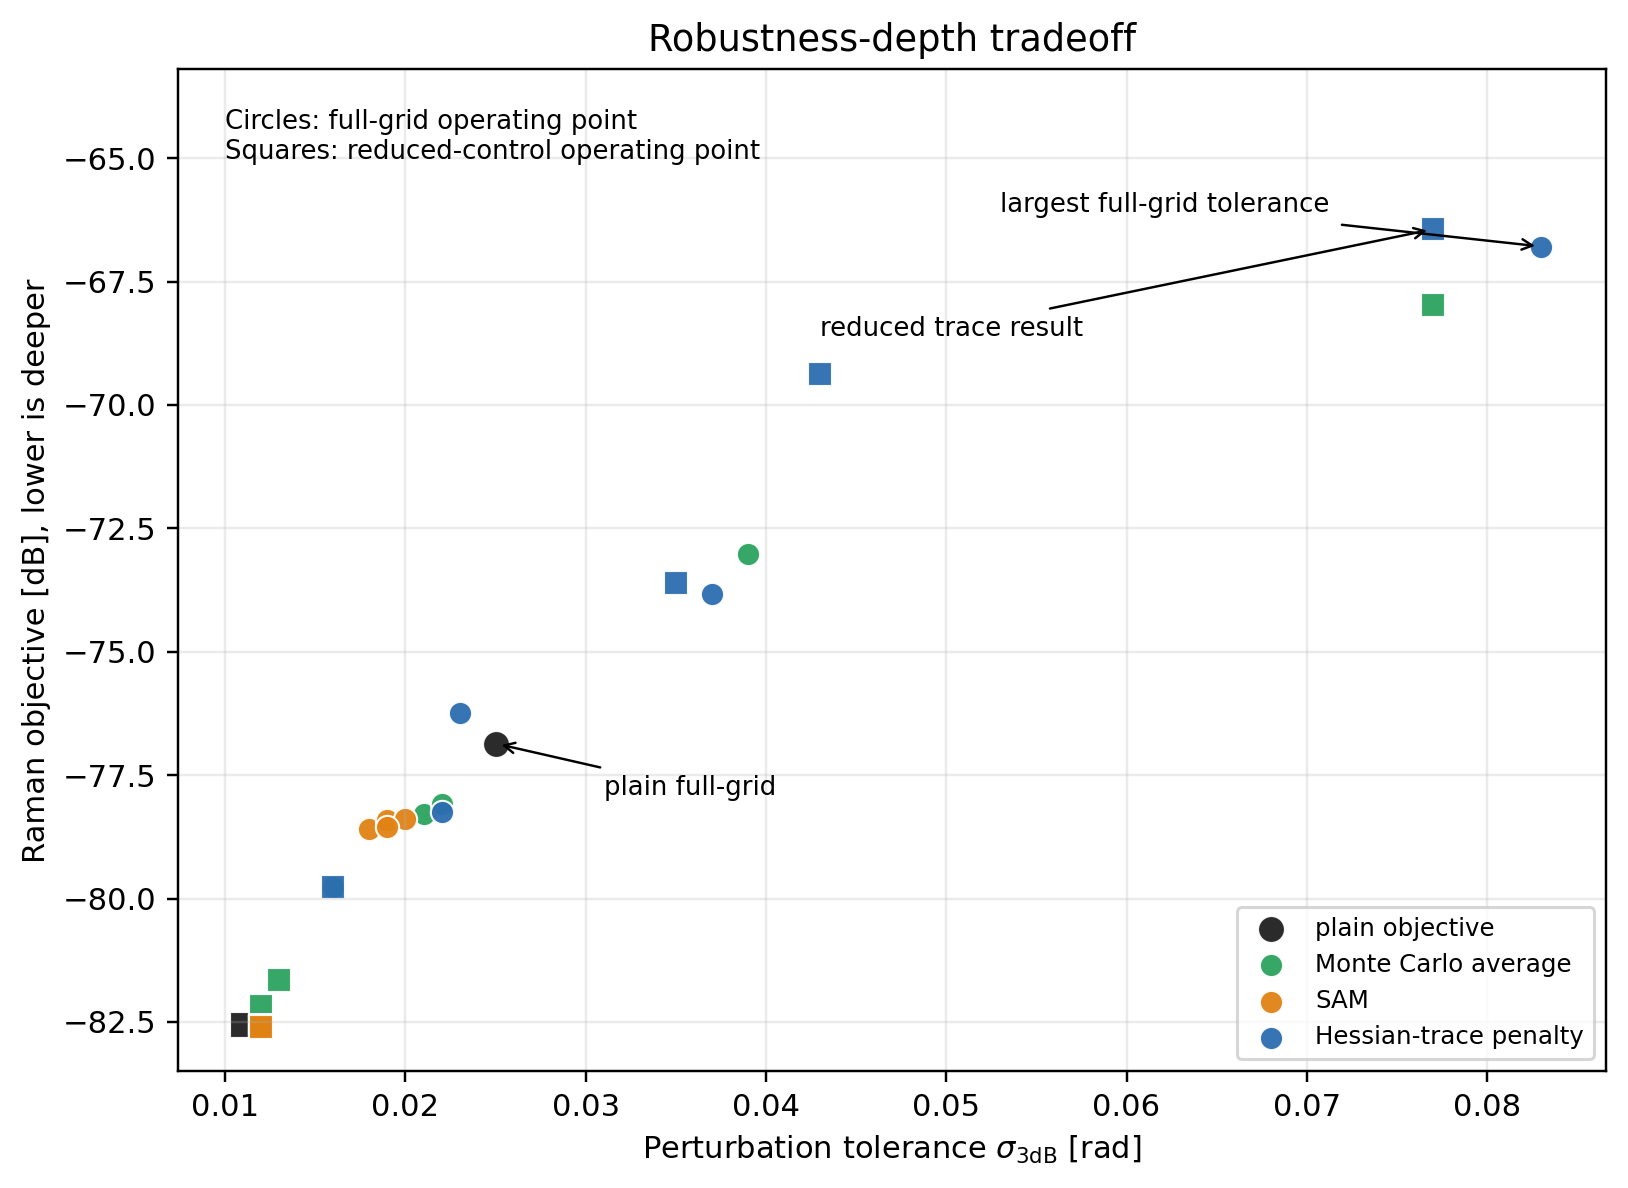
\includegraphics[width=0.92\linewidth]{figures/robustness_depth_tradeoff.png}
\caption{Depth versus perturbation tolerance. Moving right means more
tolerance to phase noise. Moving down means deeper Raman suppression. The
strongest trace-penalty cases move far to the right but lose suppression depth,
while the Monte Carlo cases give smaller tolerance gains.}
\end{figure}

\begin{figure}[H]
\centering
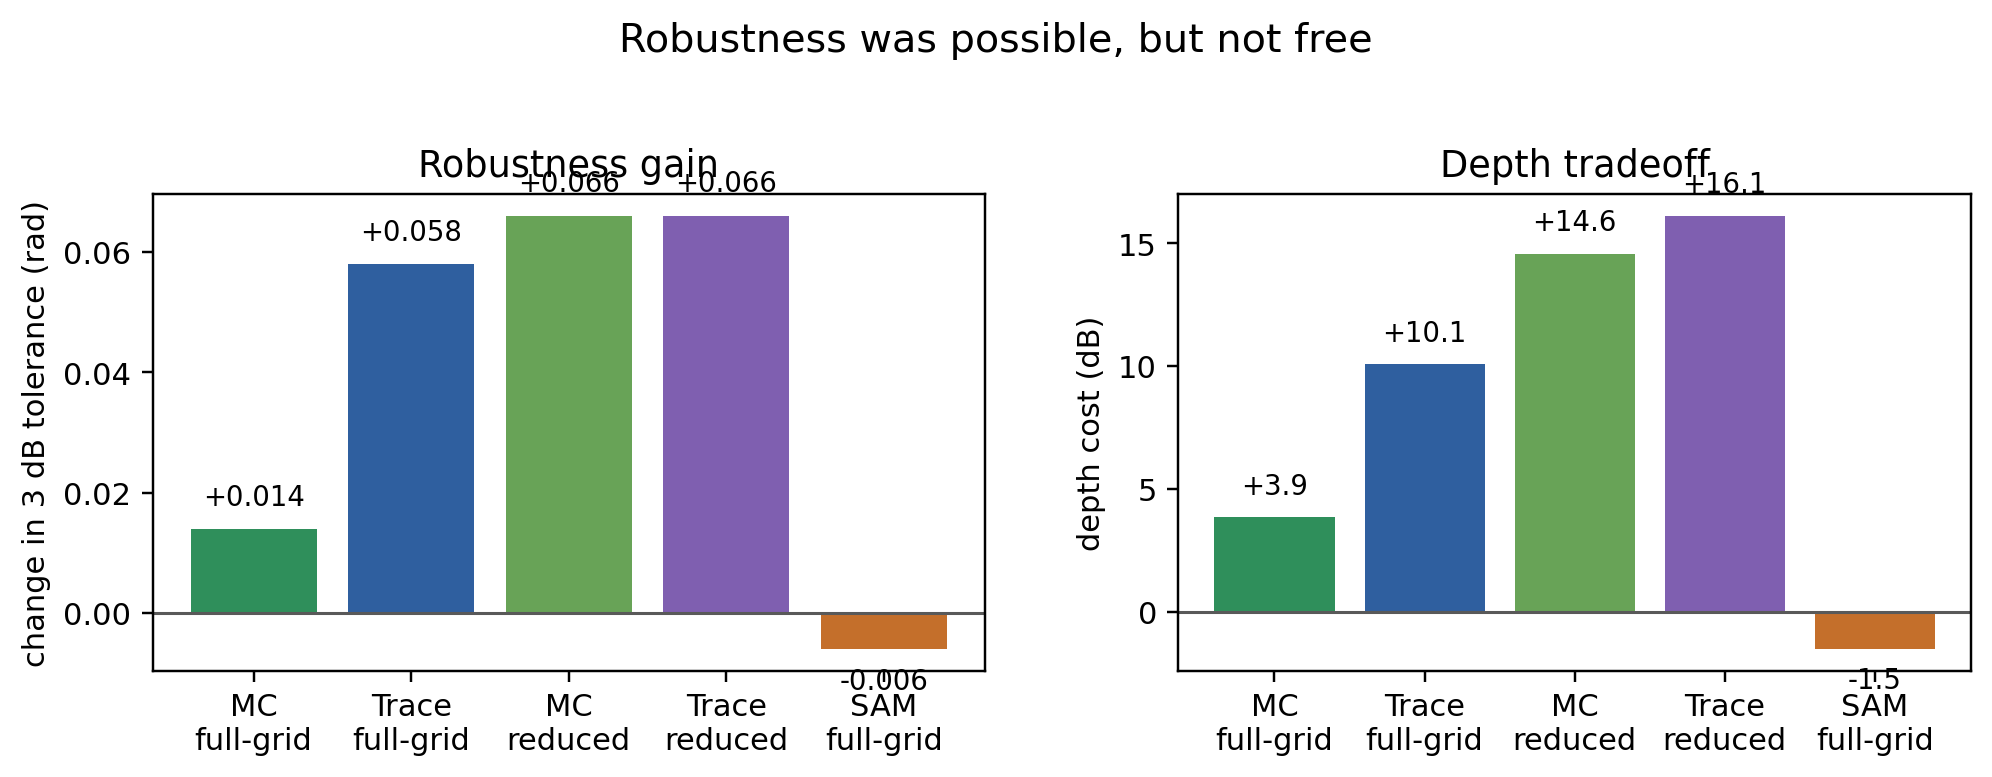
\includegraphics[width=0.92\linewidth]{figures/robustness_gain_cost_summary.png}
\caption{Robustness gain versus depth cost for representative methods. Monte
Carlo gives the cheaper full-grid improvement. The trace penalty gives the
largest tolerance gain, but the depth loss is large enough that it should not
replace the default objective.}
\end{figure}

\subsection*{Interpretive Summary}

This is a tradeoff plot, not a leaderboard with one universal winner. A point
near the lower left is deep but fragile. A point near the upper right is more
tolerant but shallower. For the current project default, depth matters enough
that the plain objective remains the reference.

\begin{figure}[H]
\centering
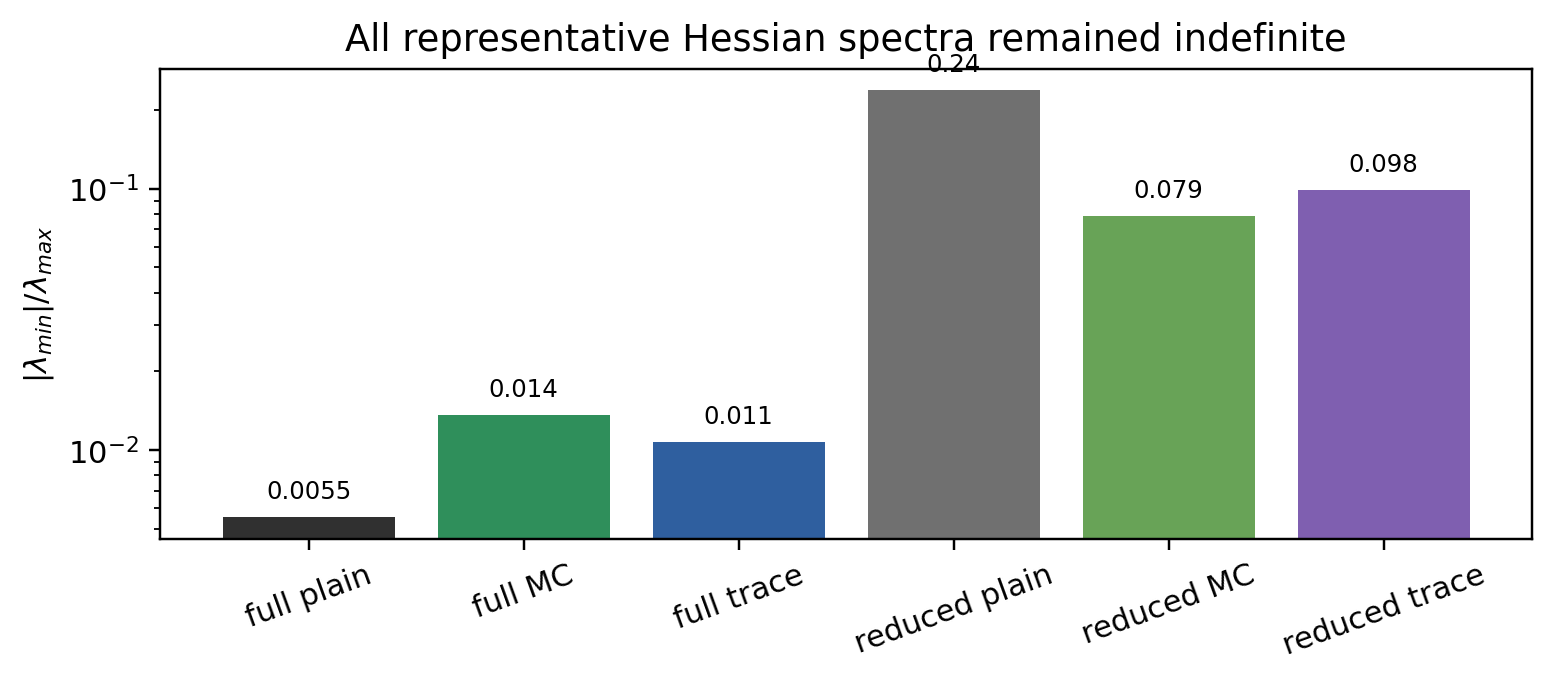
\includegraphics[width=0.78\linewidth]{figures/hessian_indefinite_summary.png}
\caption{Representative Hessian indefiniteness ratios. Each shown spectrum
has both positive and negative curvature. Robustness penalties changed
tolerance, but they did not turn the tested optima into positive-definite
local minima.}
\end{figure}

\clearpage
\section{Representative Results}

The following pages use the standard research-note format: first the phase
diagnostic, then the matching spectral-evolution heat map on the same page.
Read each robustness case against the no-optimization control and the plain
objective reference.

\subsection*{How To Read These Pages}

\textbf{Phase diagnostic.} The diagnostic shows the applied phase, unwrapped
phase, group delay, group-delay dispersion, and instantaneous frequency shift.
Large spikes or rapid oscillations are warning signs that a mask may be
difficult to implement experimentally.

\textbf{Spectral-evolution heat map.} The heat map shows how spectral power
changes along the fiber. It is the best quick visual check for whether a phase
mask changed the physical evolution or merely produced a different-looking
input phase.

\textbf{Control comparison.} The no-optimization page is the control group.
The plain objective page is the depth reference. The Monte Carlo and trace
pages should be judged by the depth-versus-tolerance tradeoff, not by depth
alone.

\subsection*{Intuition Check}

The phase diagnostic is the input story. The heat map is the fiber-response
story. A robustness claim needs both, plus the scalar tolerance number.

\clearpage

\begin{figure}[H]
\centering

\includegraphics[height=0.47\textheight]{figures/no_optimization_phase_diagnostic.png}
\vspace{0.5em}

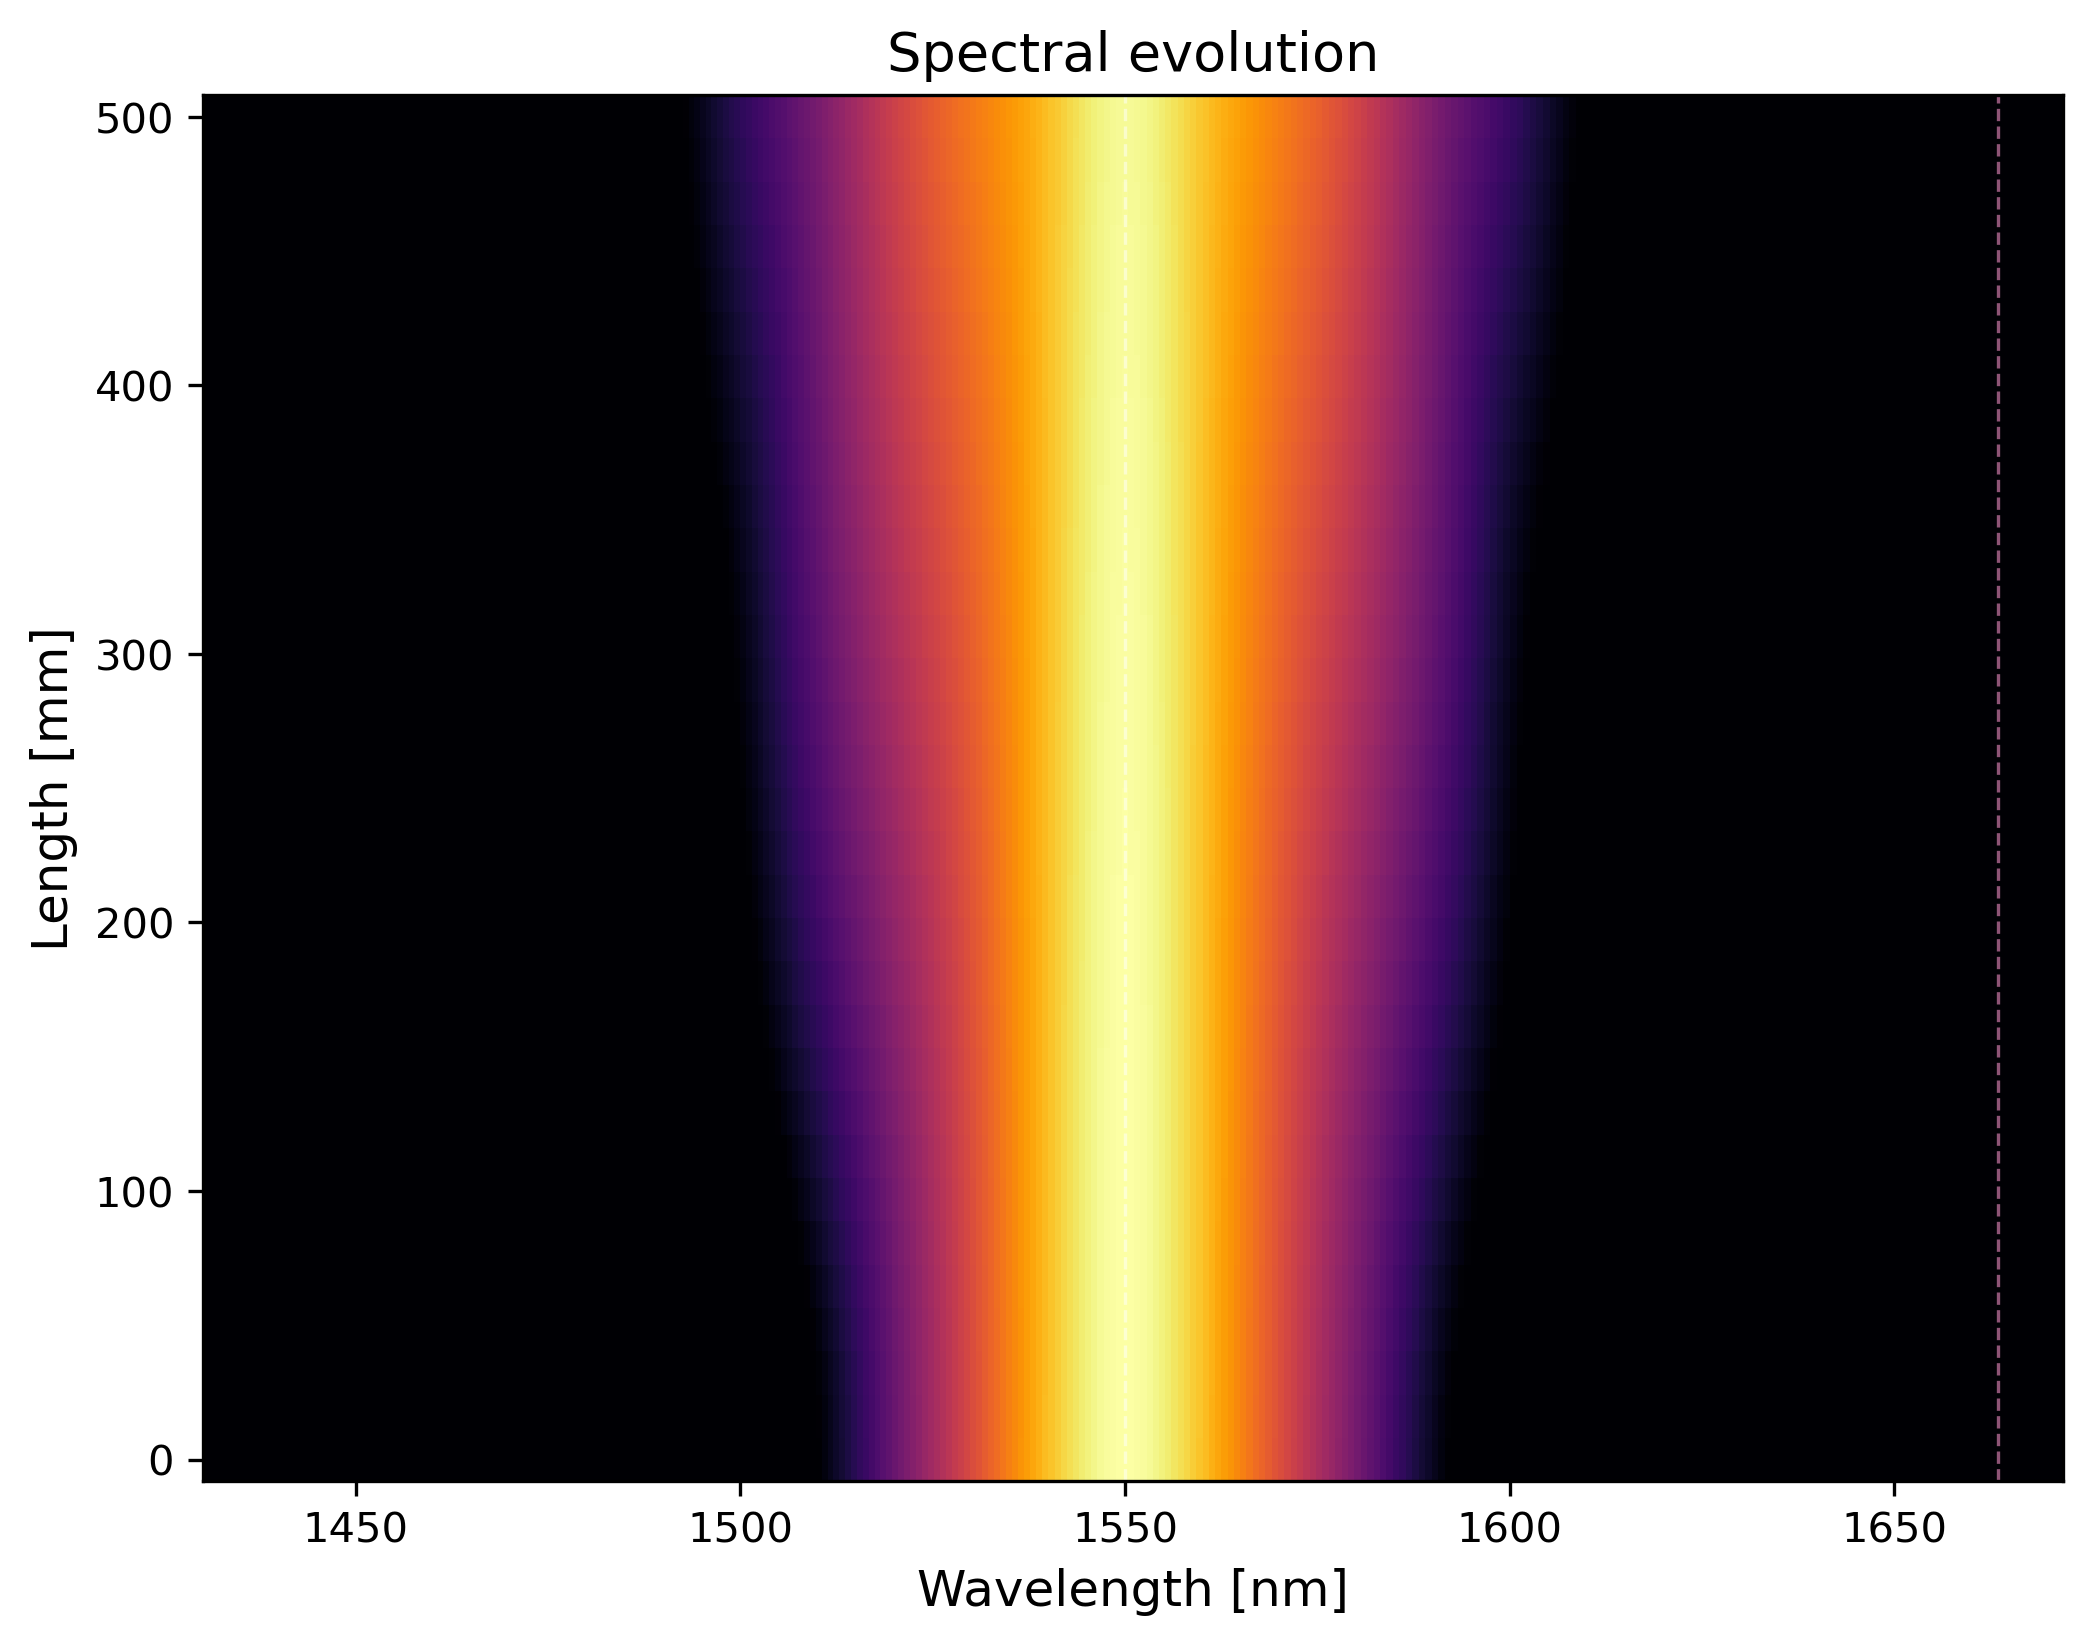
\includegraphics[height=0.31\textheight]{figures/canonical_unshaped_evolution.png}
\caption{No-optimization control. The left diagnostic has flat applied phase;
the heat map shows the unshaped propagation for the full-grid operating point.
This page is the reference before any sharpness or robustness objective
is allowed to change the phase.}
\end{figure}

\begin{figure}[H]
\centering
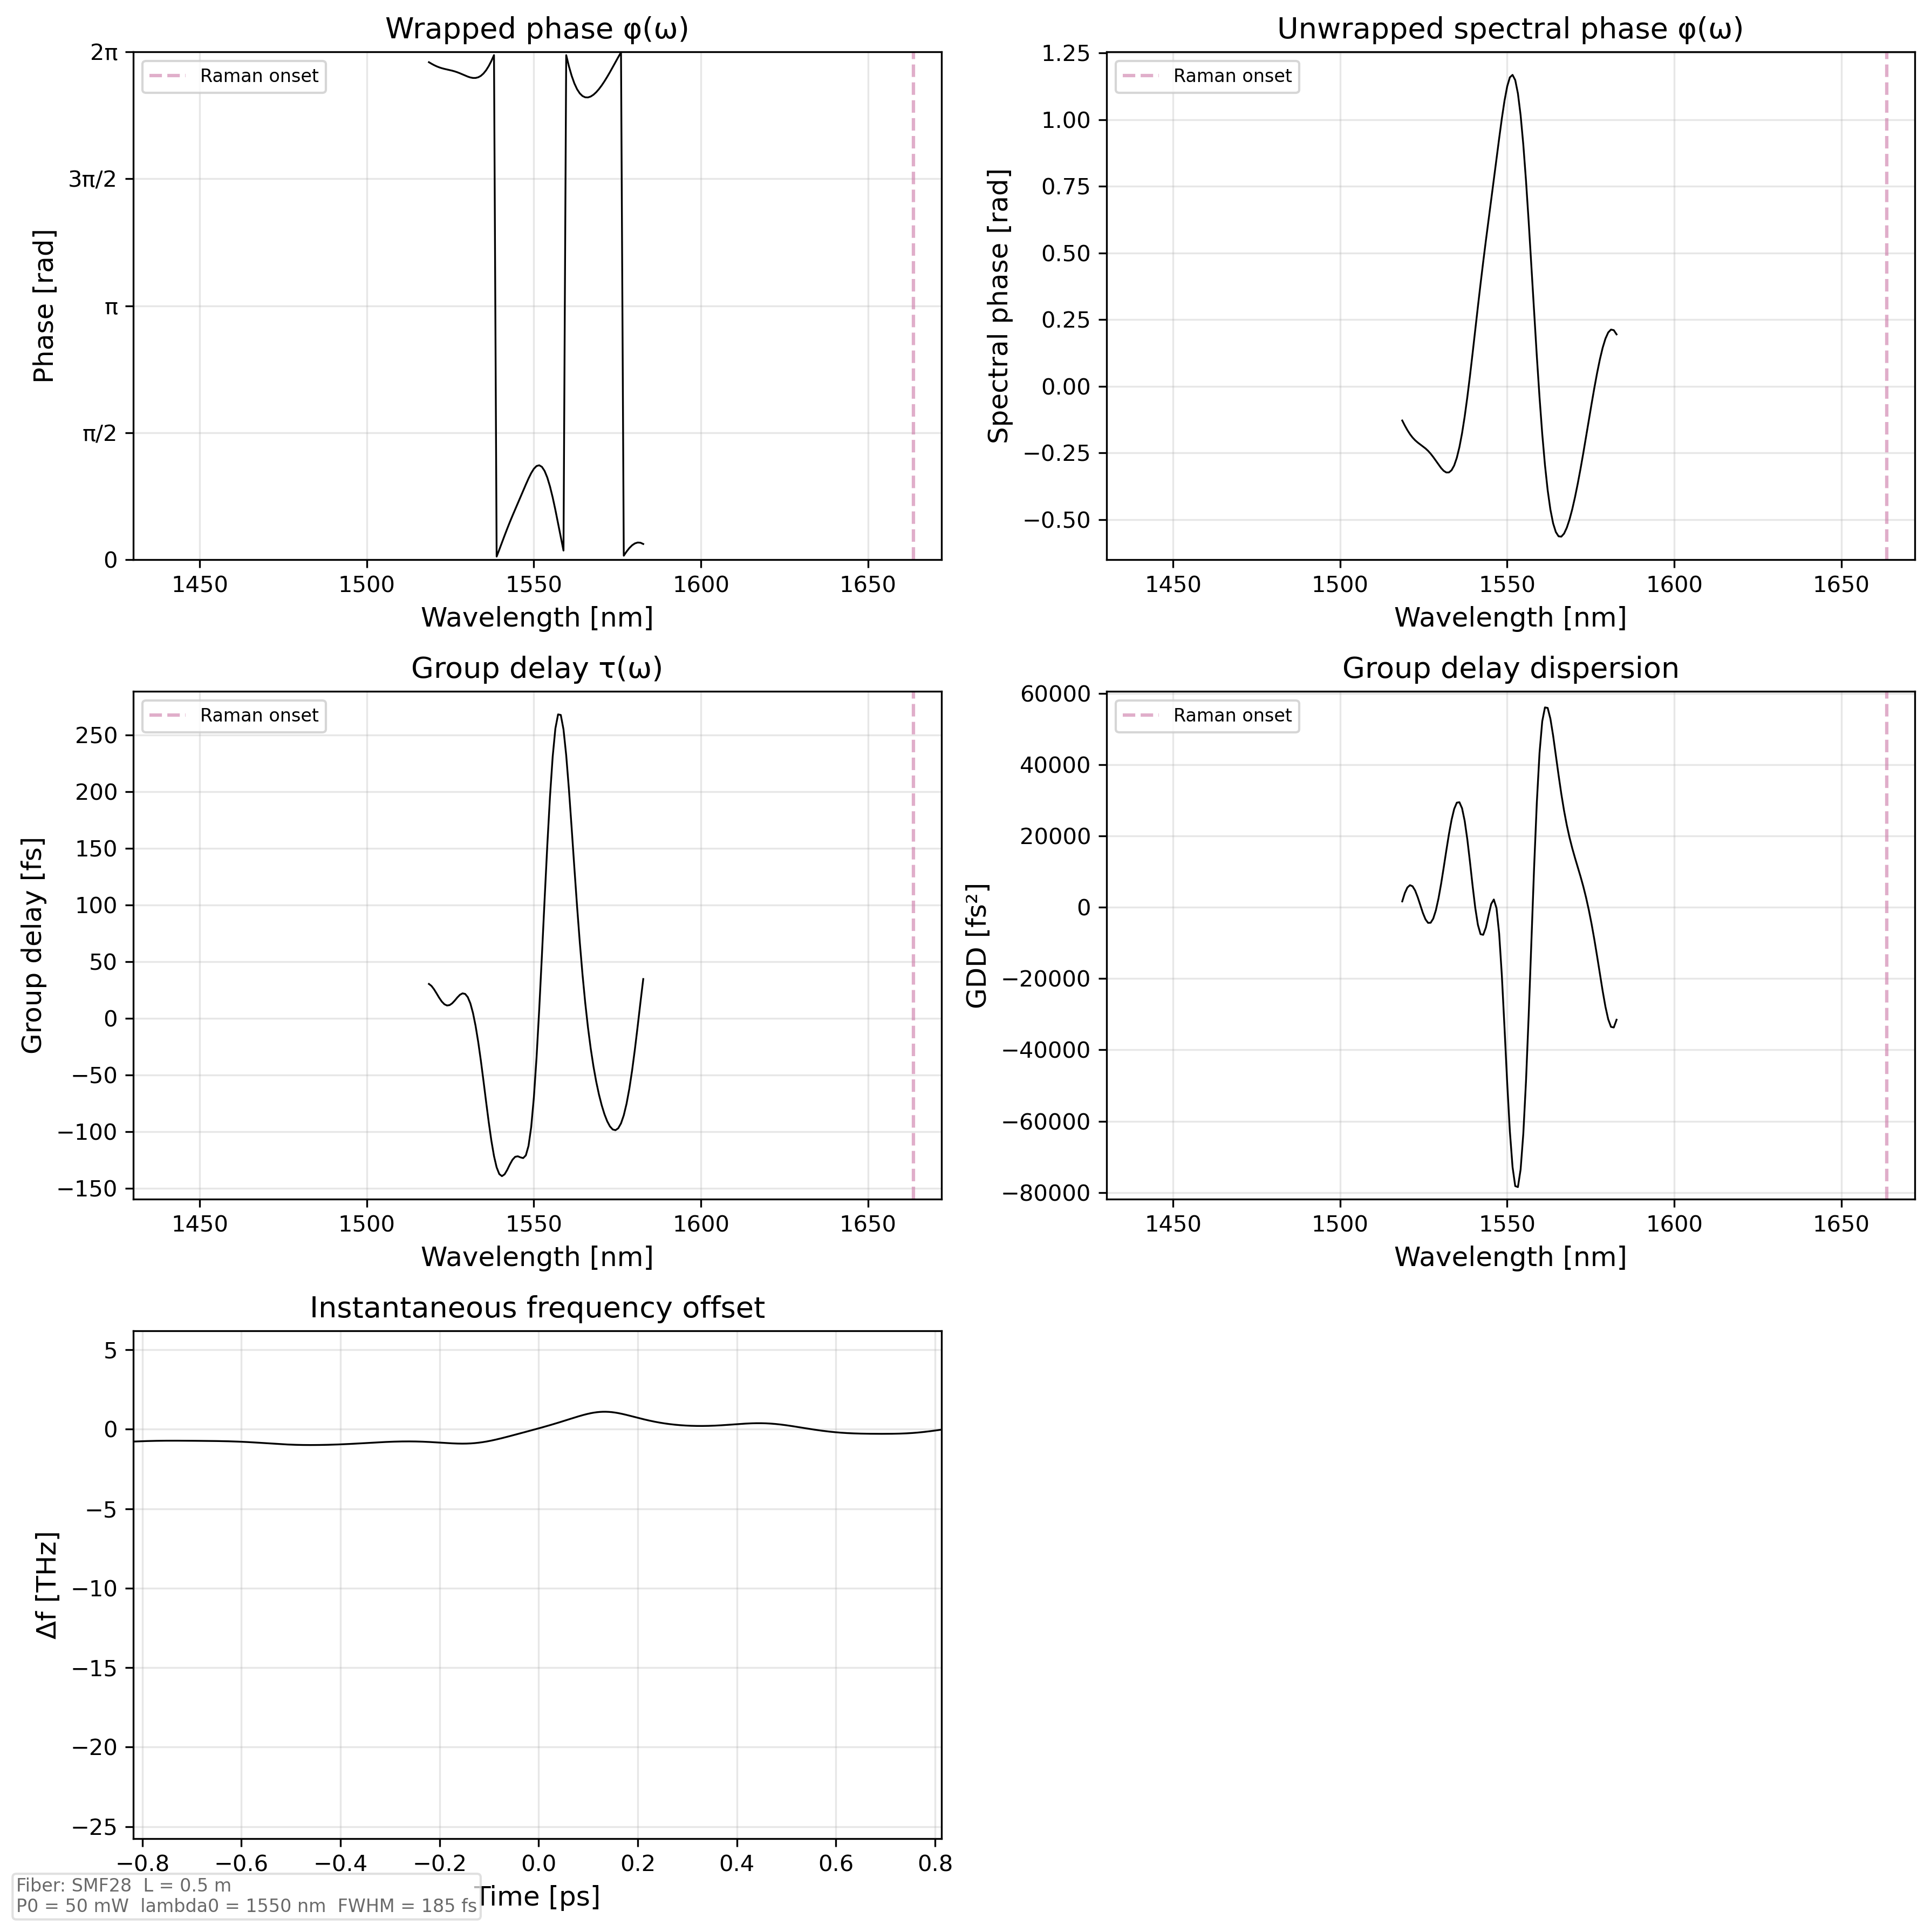
\includegraphics[height=0.47\textheight]{figures/canonical_plain_phase_diagnostic.png}
\vspace{0.5em}

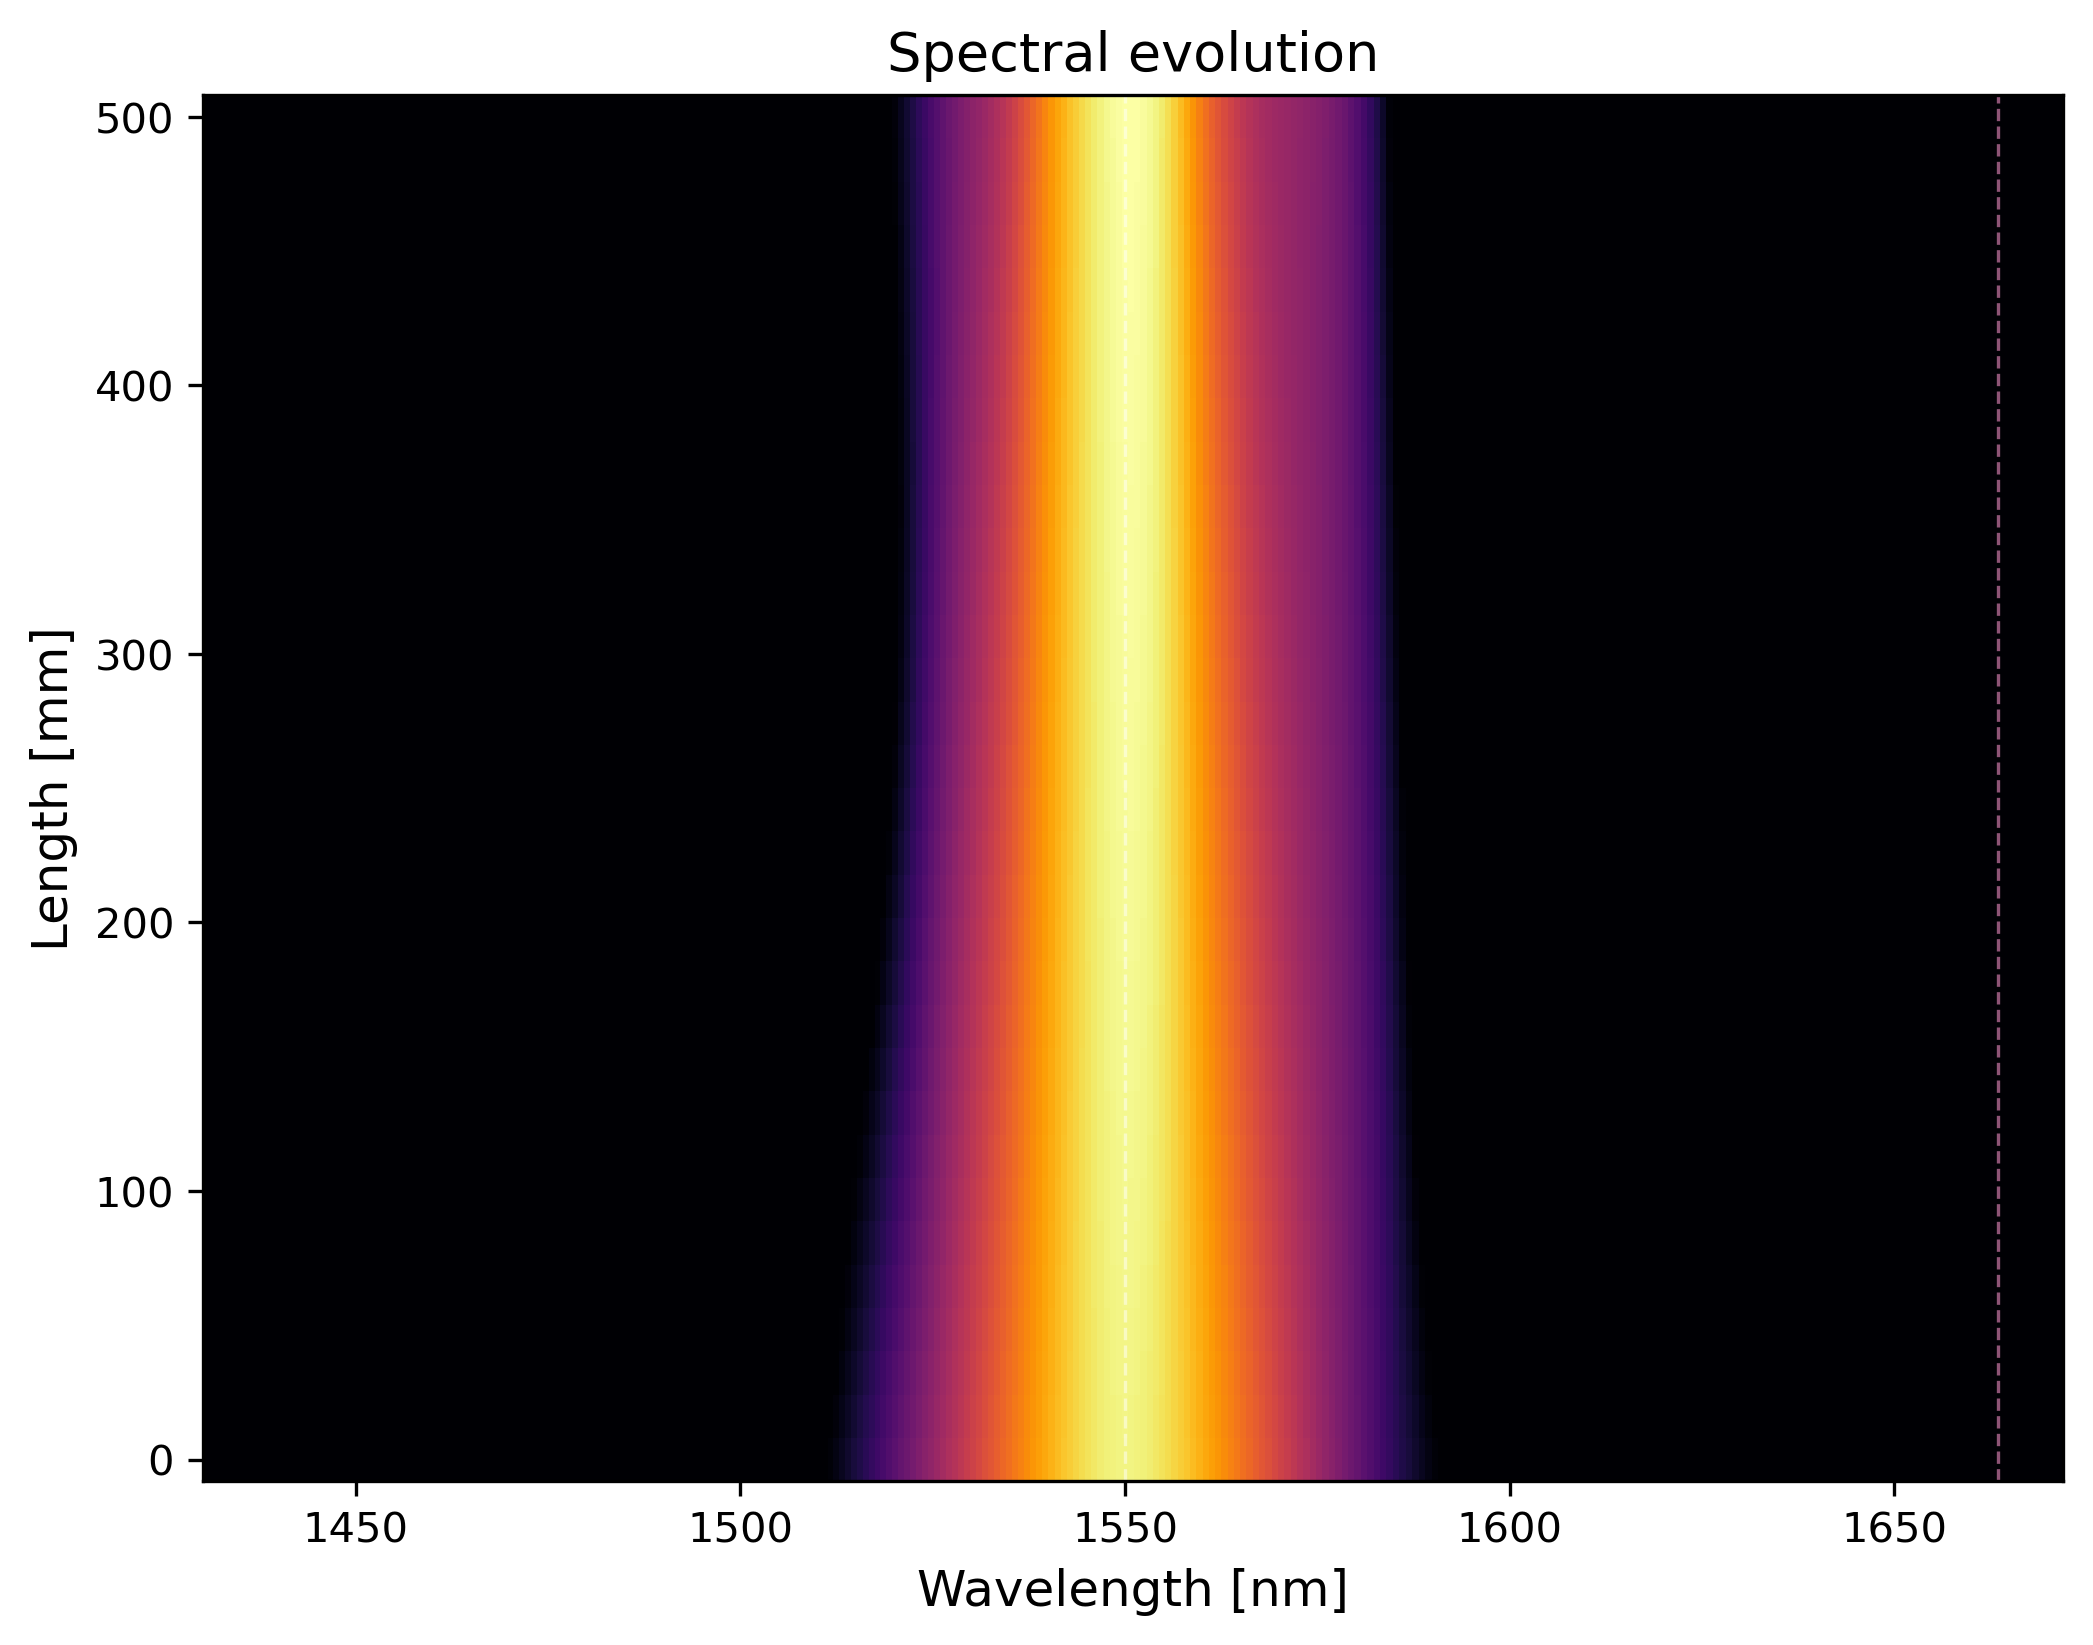
\includegraphics[height=0.31\textheight]{figures/canonical_plain_evolution.png}
\caption{Plain full-grid objective. This solution reached about
\(-76.86\,\mathrm{dB}\) with \(\sigmathreedb\approx0.025\,\mathrm{rad}\). It
is the depth-oriented reference case for this note.}
\end{figure}

\begin{figure}[H]
\centering
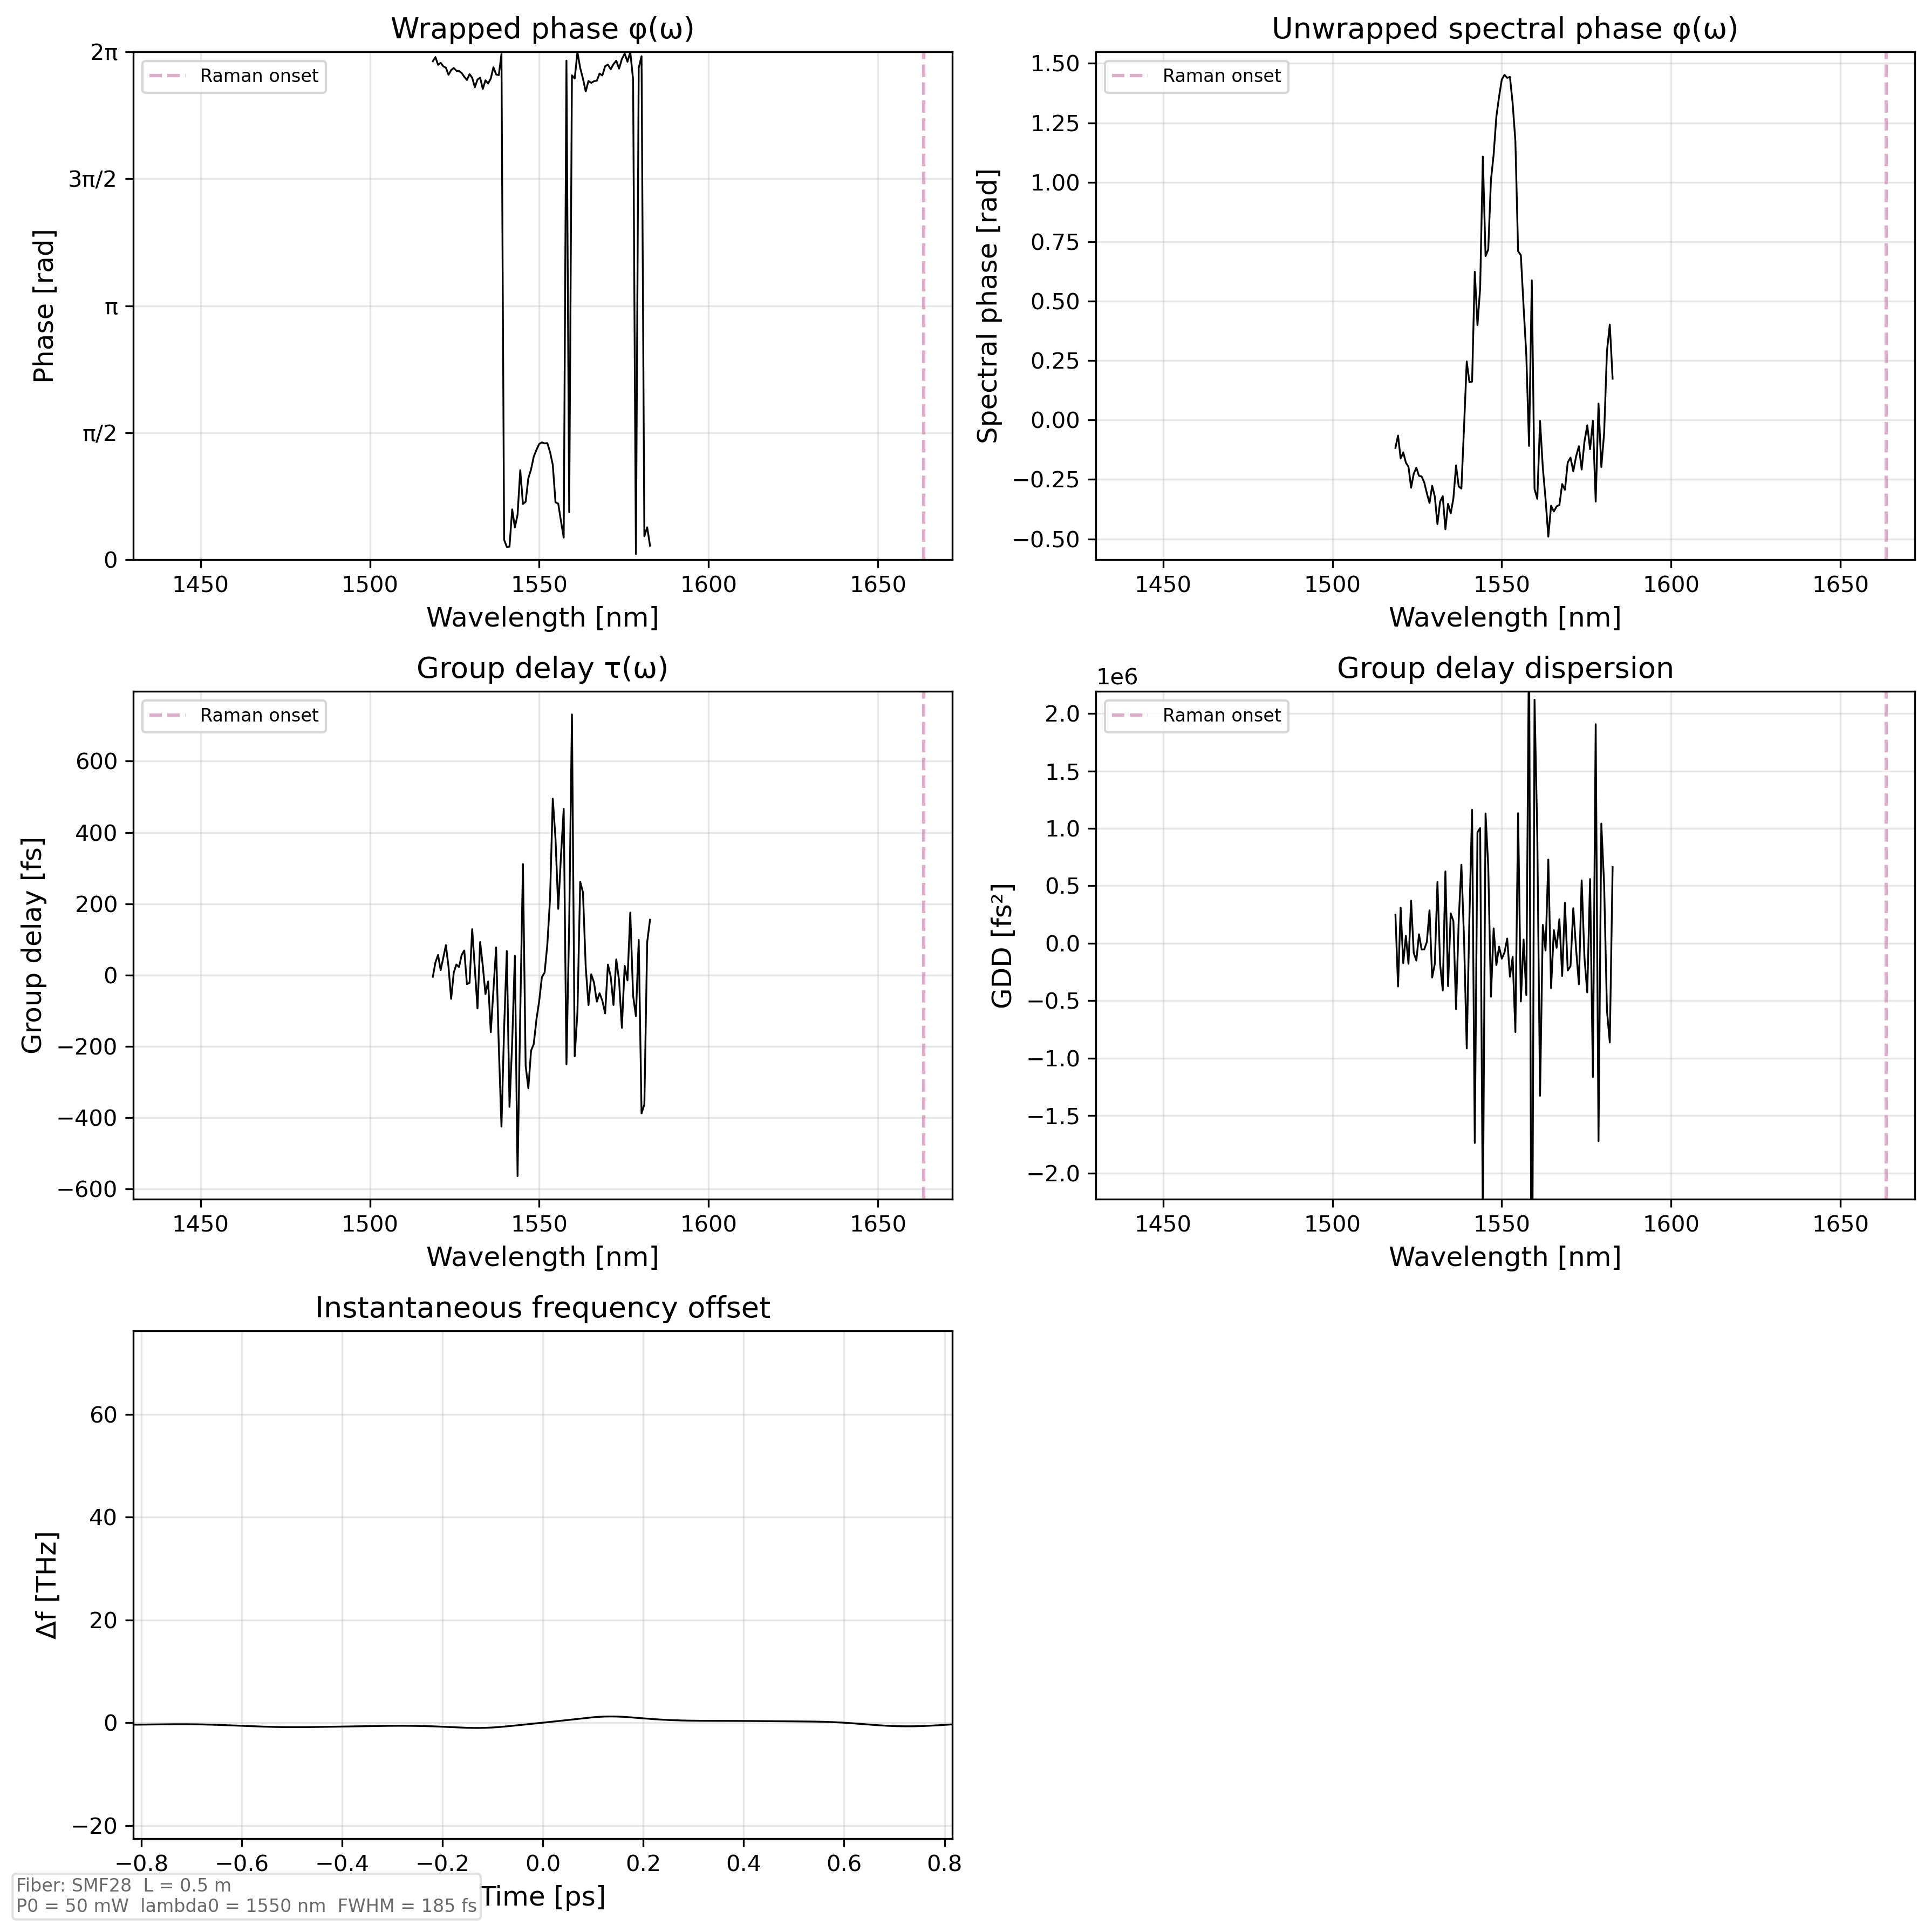
\includegraphics[height=0.47\textheight]{figures/canonical_mc_phase_diagnostic.png}
\vspace{0.5em}

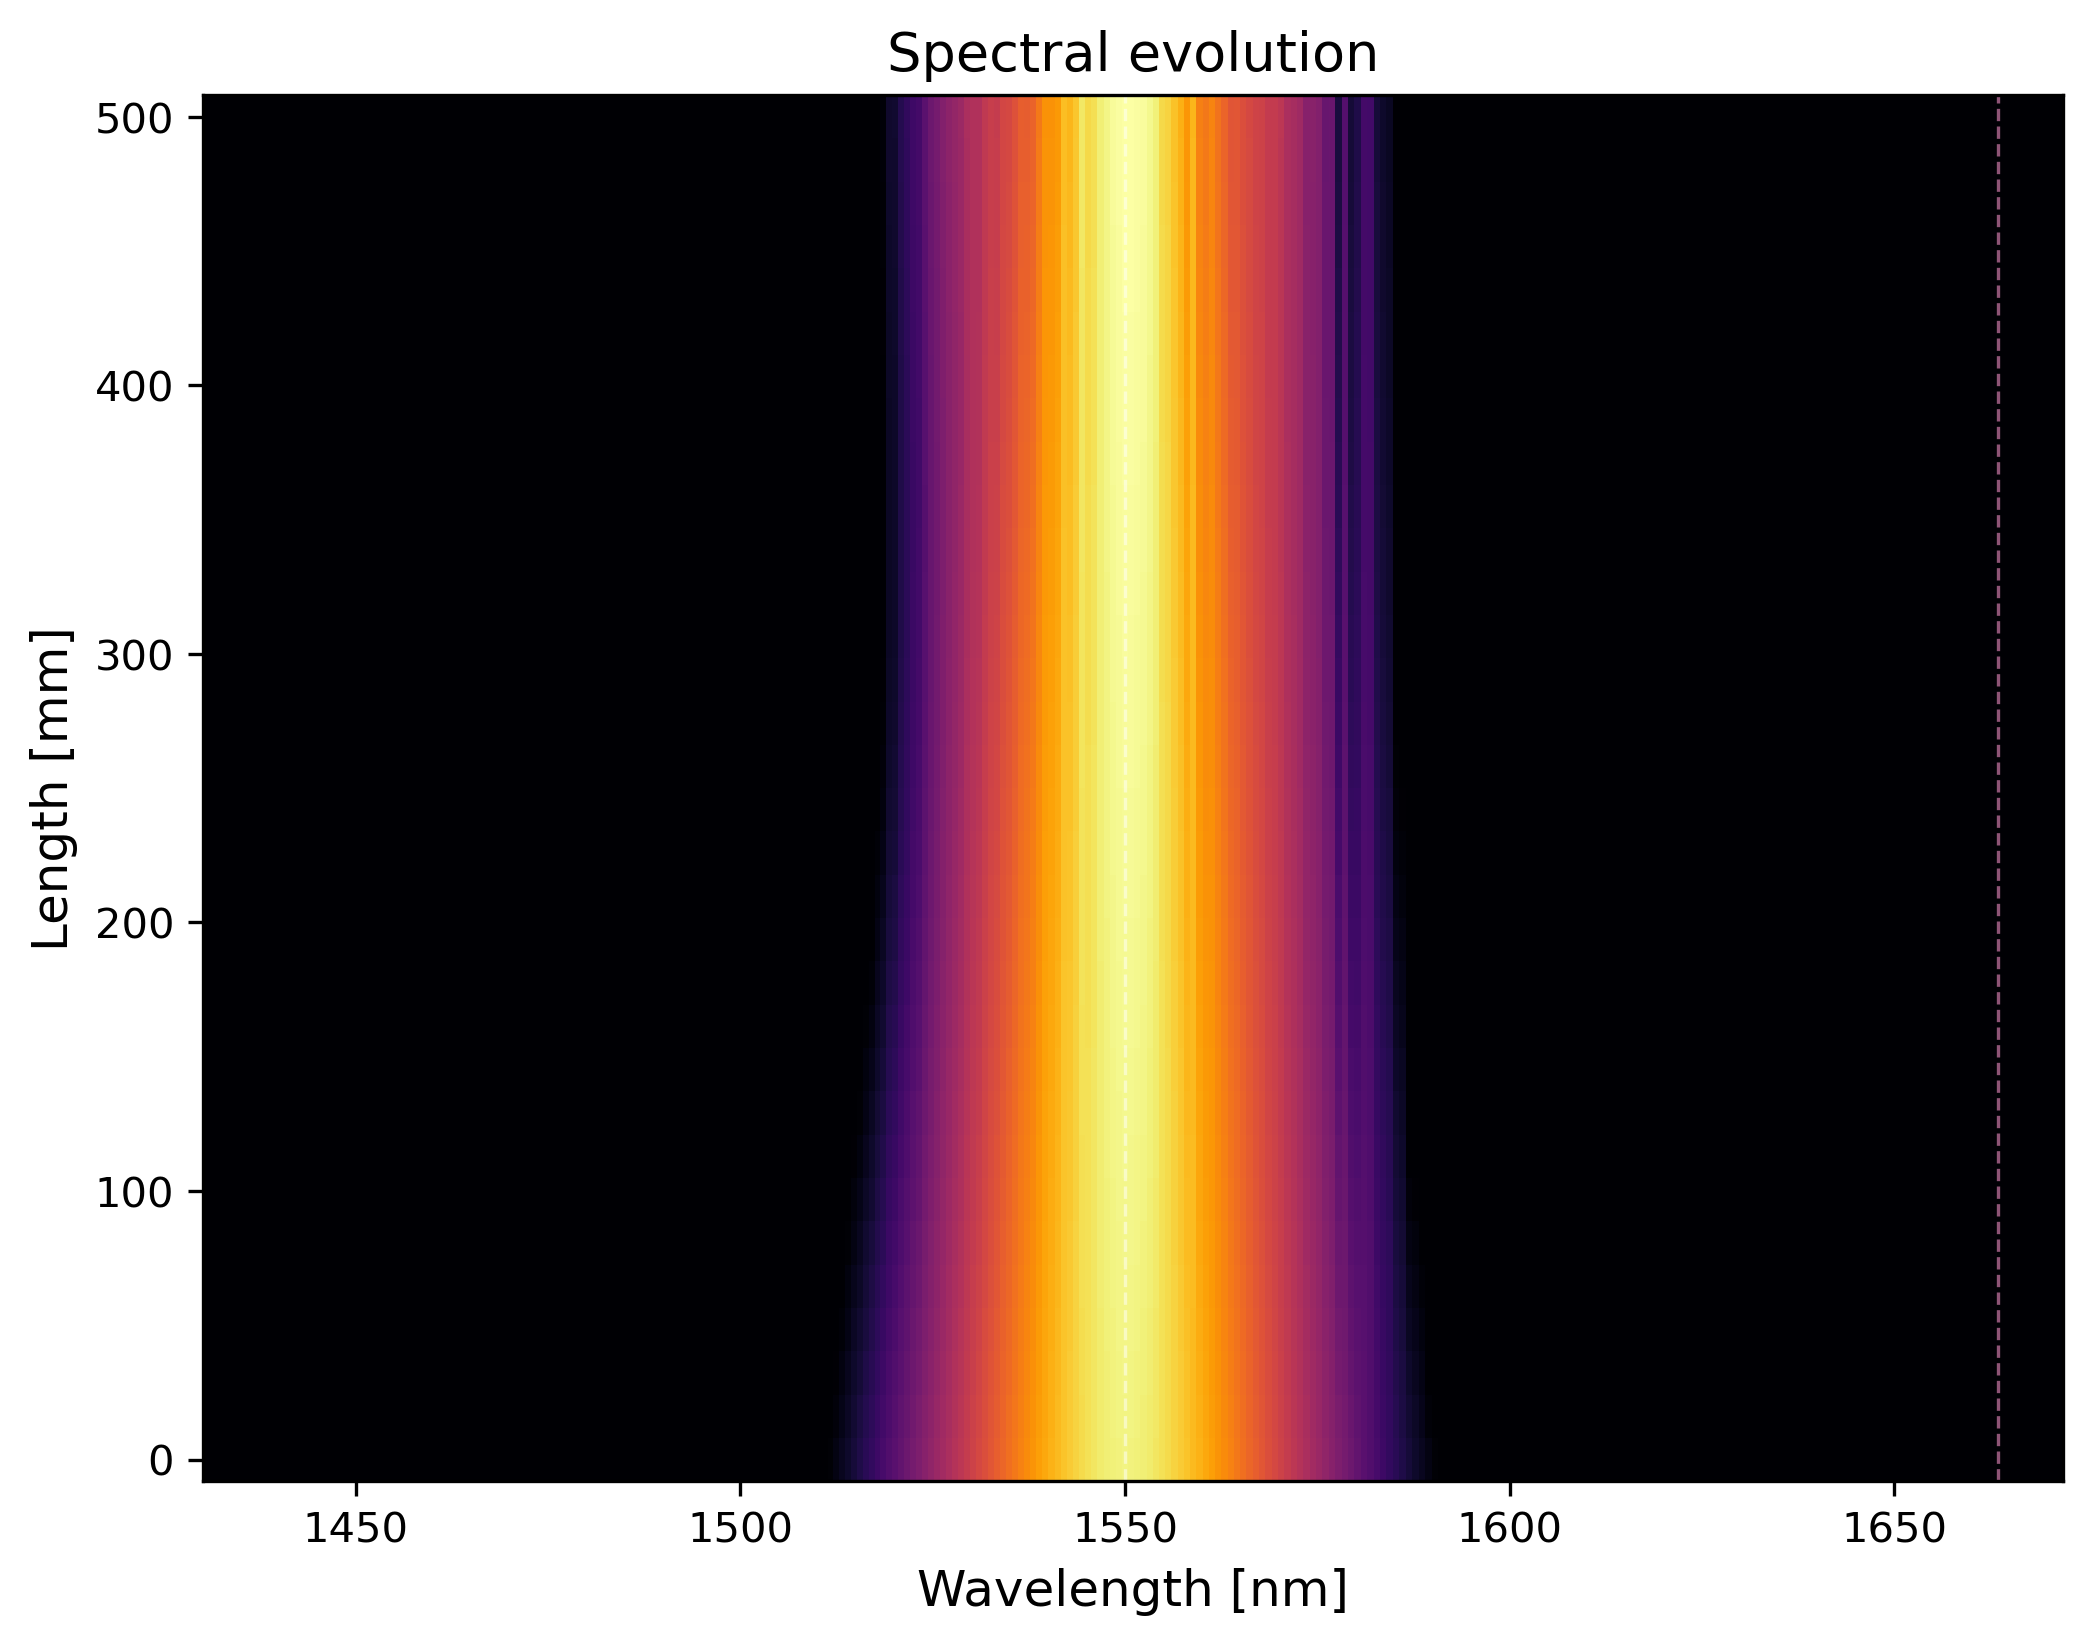
\includegraphics[height=0.31\textheight]{figures/canonical_mc_evolution.png}
\caption{Monte Carlo phase-averaged objective on the full-grid operating
point. The strongest tested MC case reached about \(-73.01\,\mathrm{dB}\) with
\(\sigmathreedb\approx0.039\,\mathrm{rad}\), improving tolerance by about
\(0.014\,\mathrm{rad}\) at a depth cost of about \(3.85\,\mathrm{dB}\).}
\end{figure}

\begin{figure}[H]
\centering
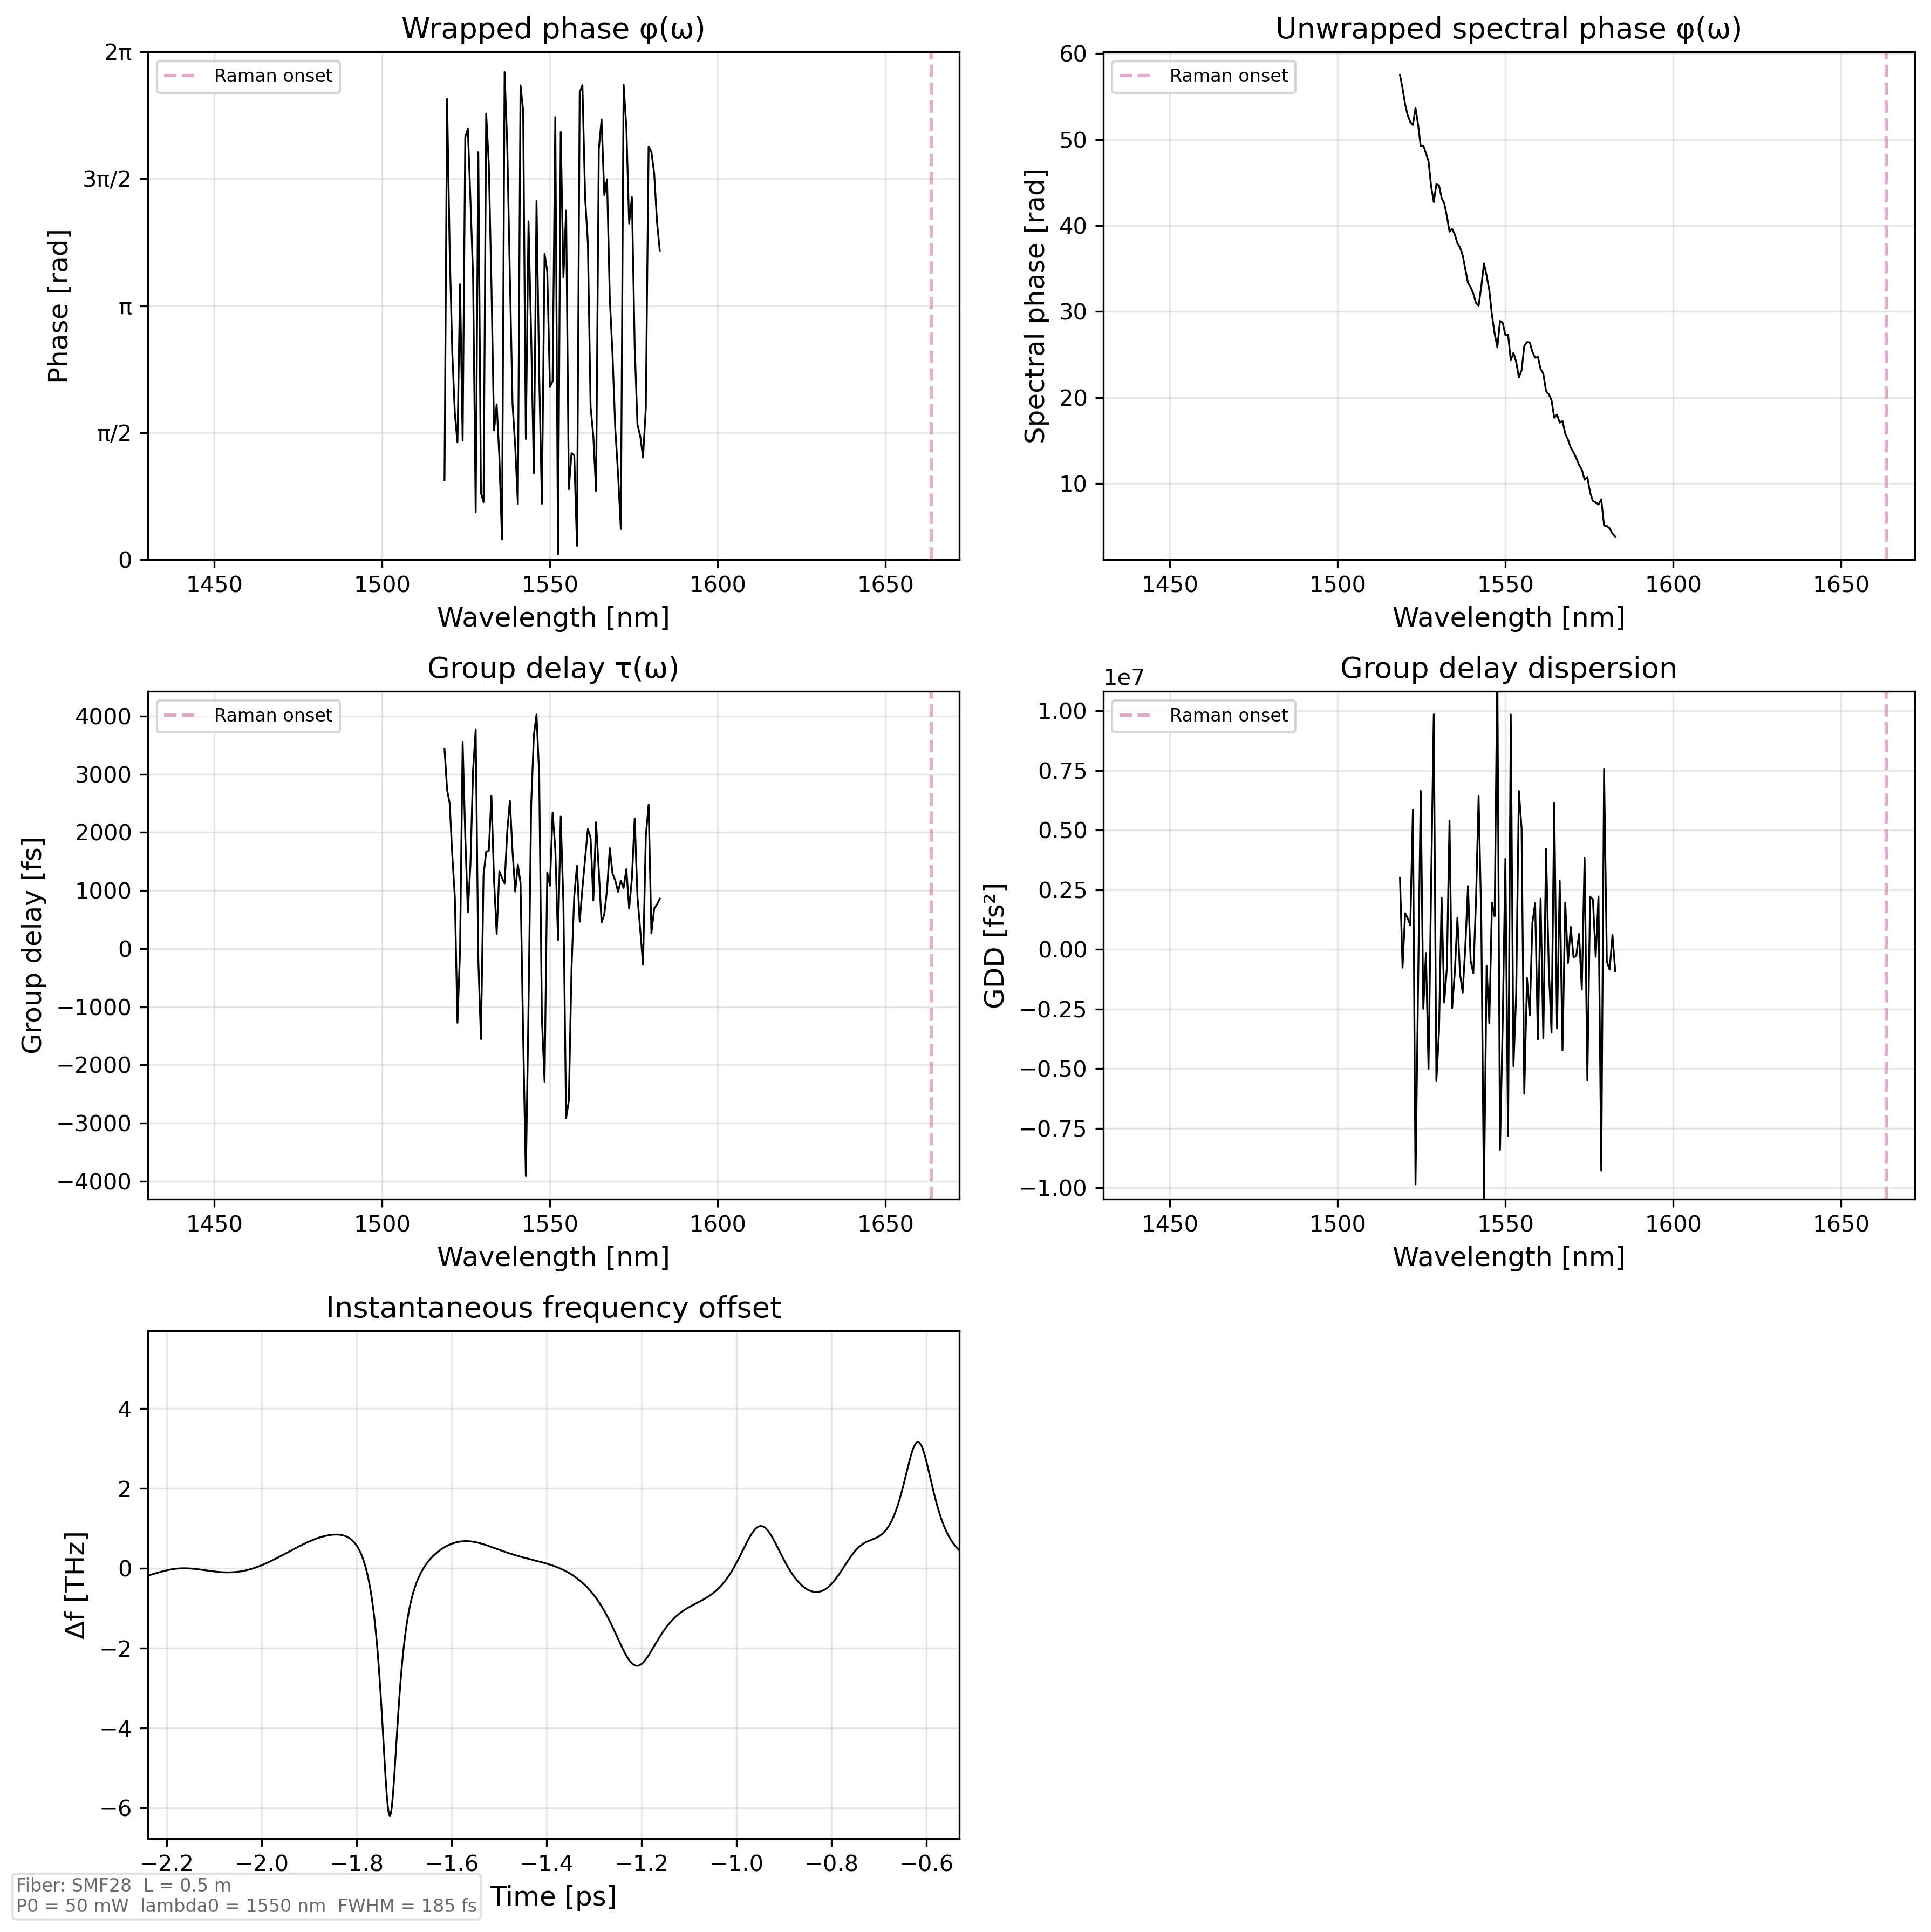
\includegraphics[height=0.47\textheight]{figures/canonical_trace_phase_diagnostic.png}
\vspace{0.5em}

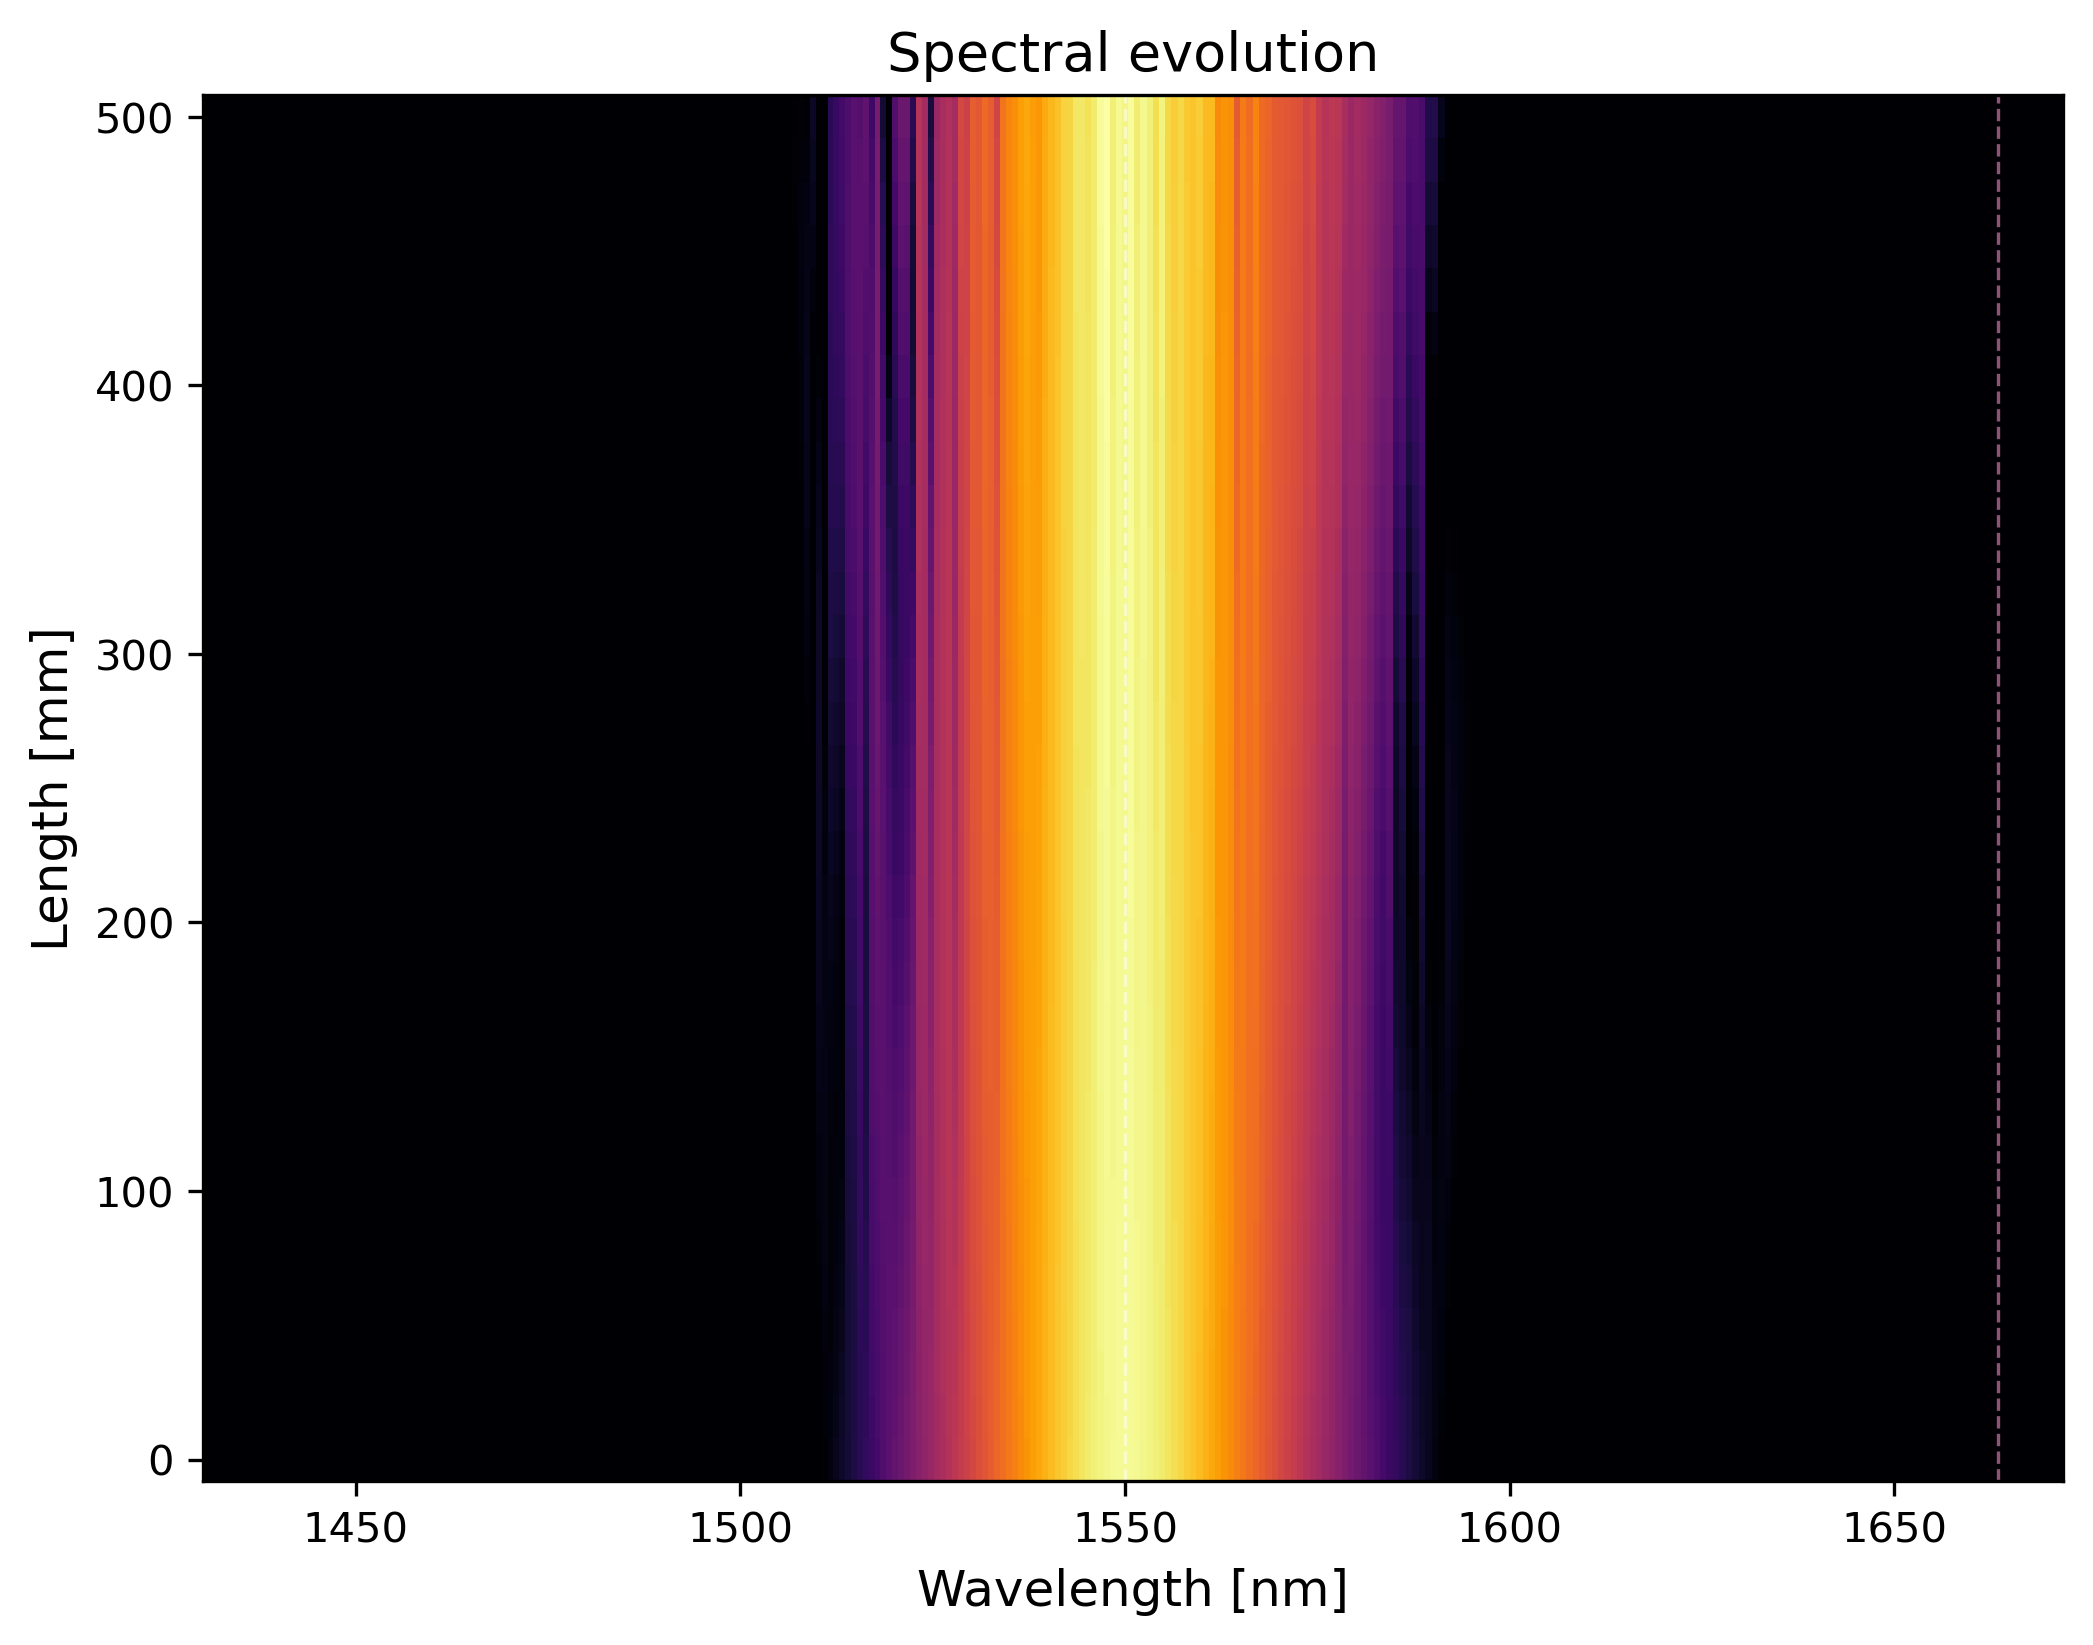
\includegraphics[height=0.31\textheight]{figures/canonical_trace_evolution.png}
\caption{Hessian-trace penalty on the full-grid operating point. This case
reached about \(-66.79\,\mathrm{dB}\) with
\(\sigmathreedb\approx0.083\,\mathrm{rad}\). It gives the largest full-grid
tolerance gain, but the depth cost is about \(10.08\,\mathrm{dB}\).}
\end{figure}

\begin{figure}[H]
\centering
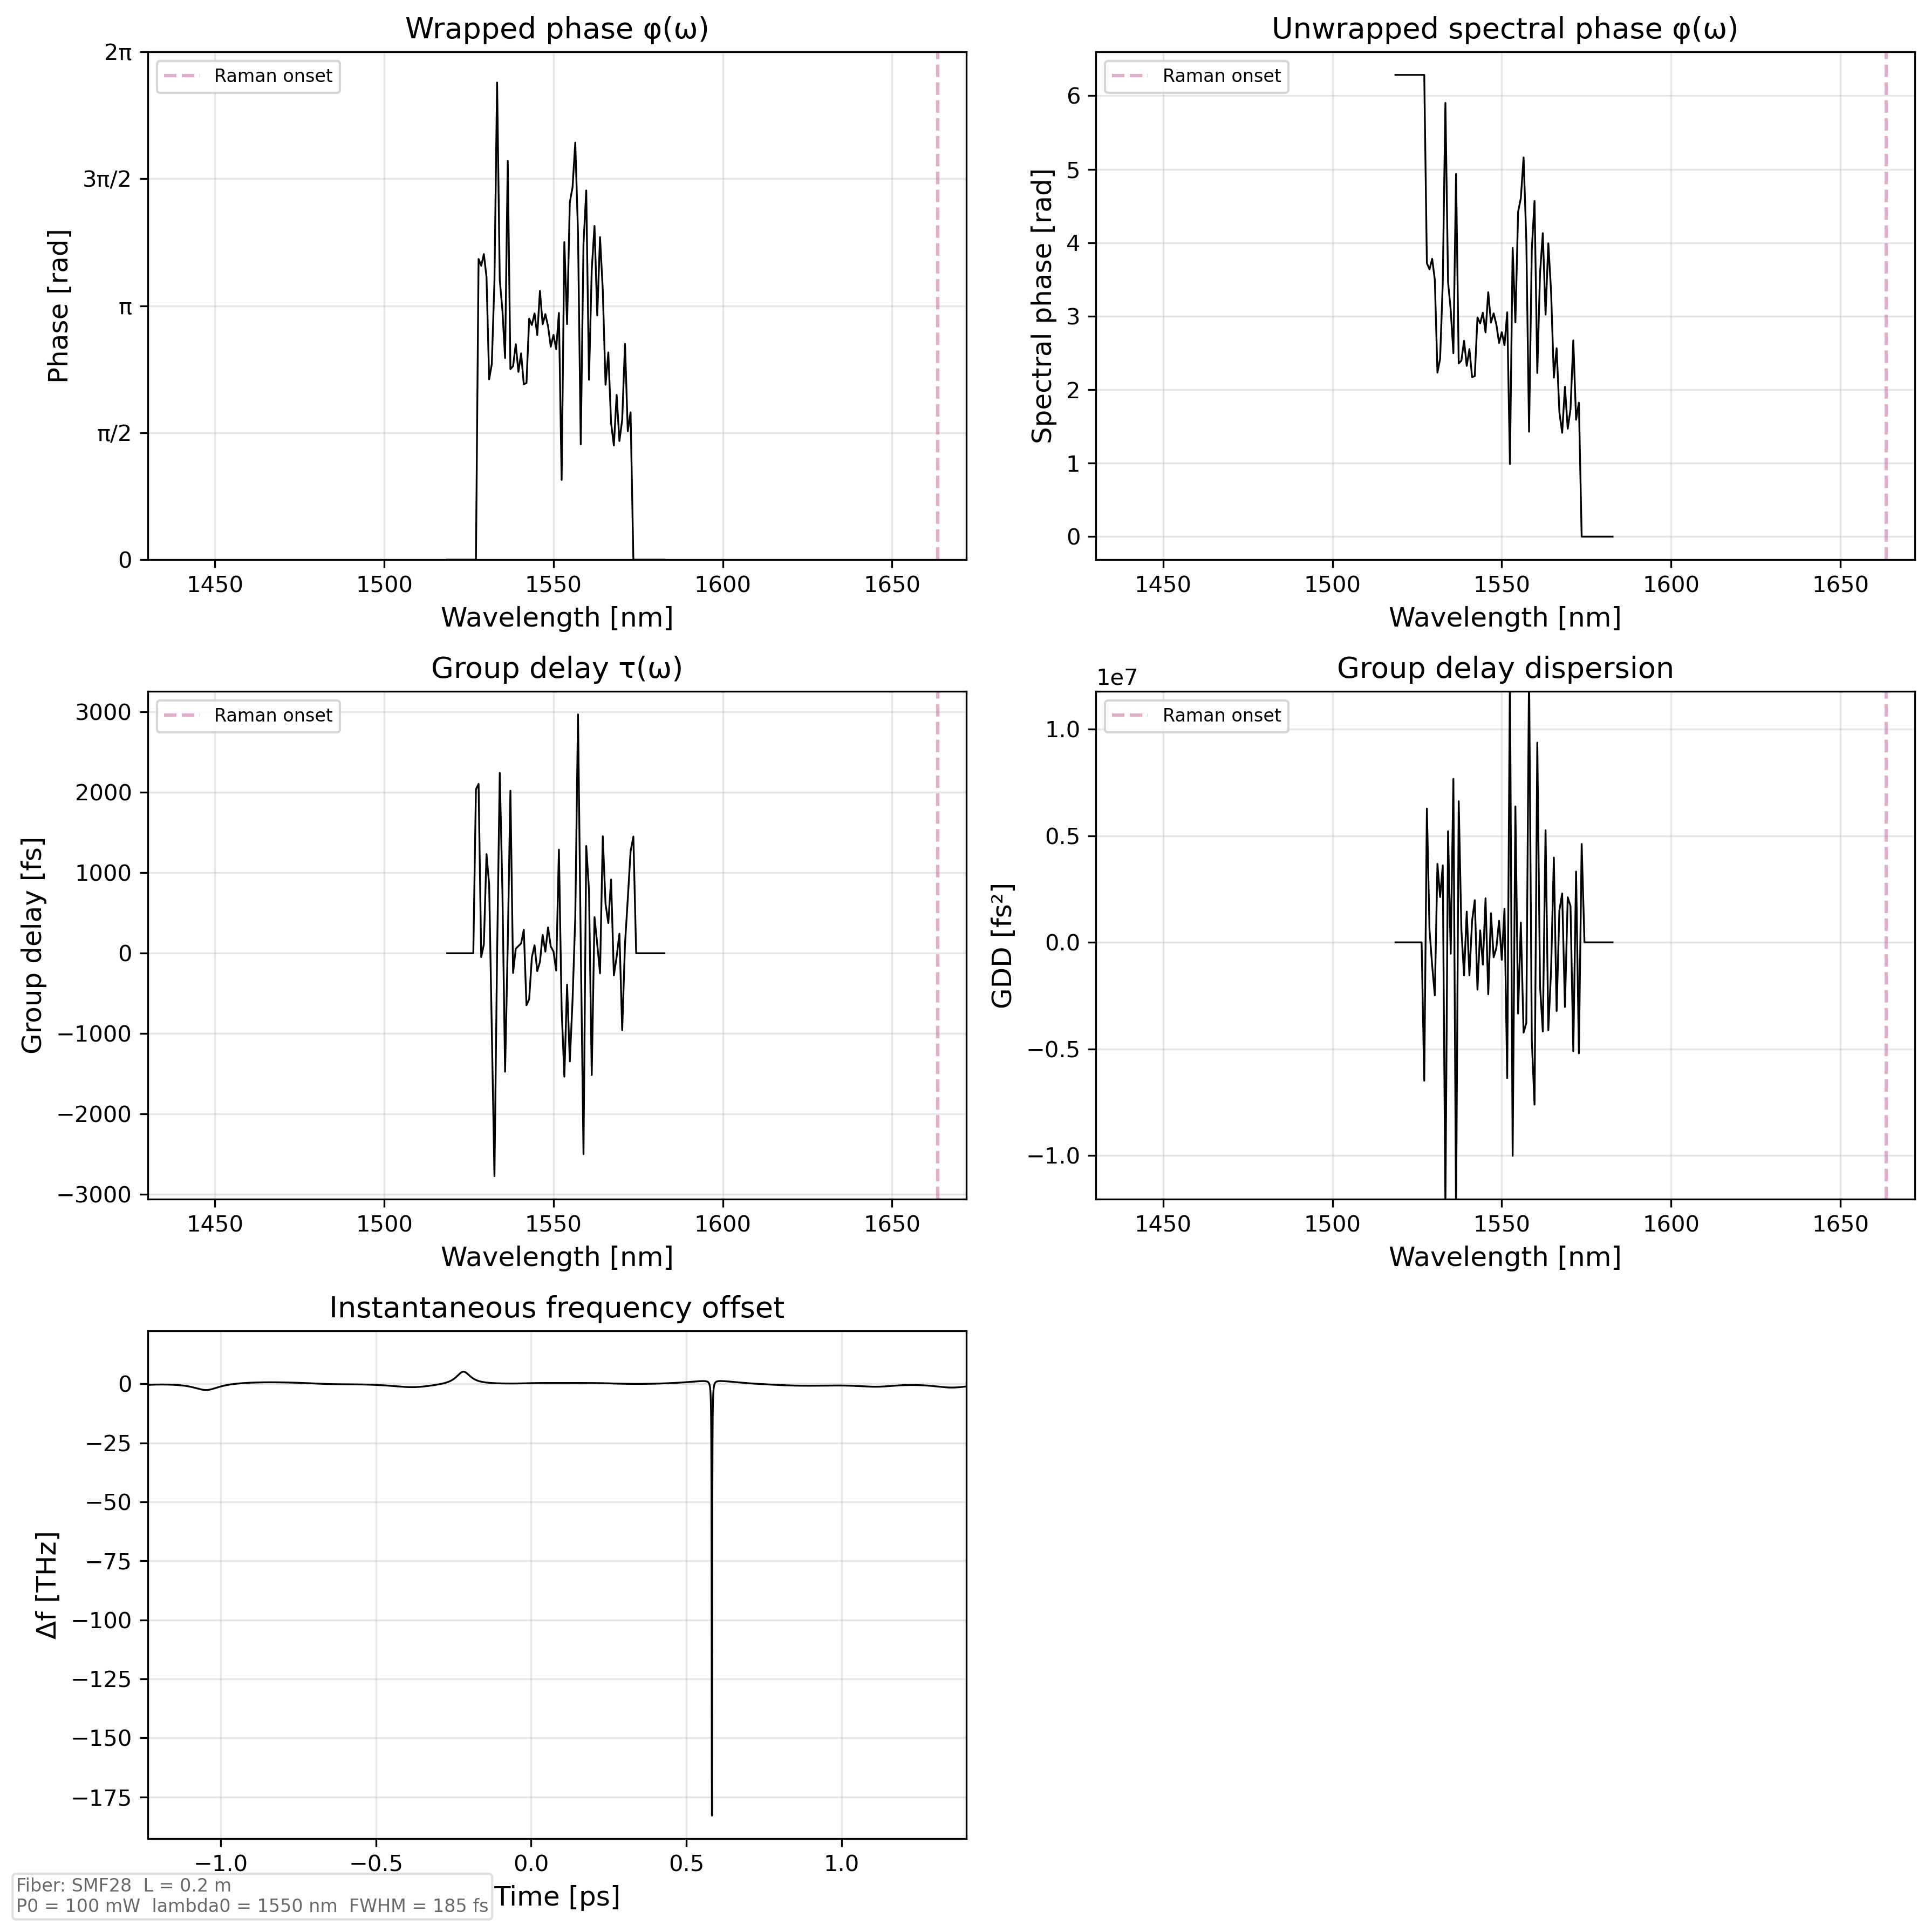
\includegraphics[height=0.47\textheight]{figures/reduced_trace_phase_diagnostic.png}
\vspace{0.5em}

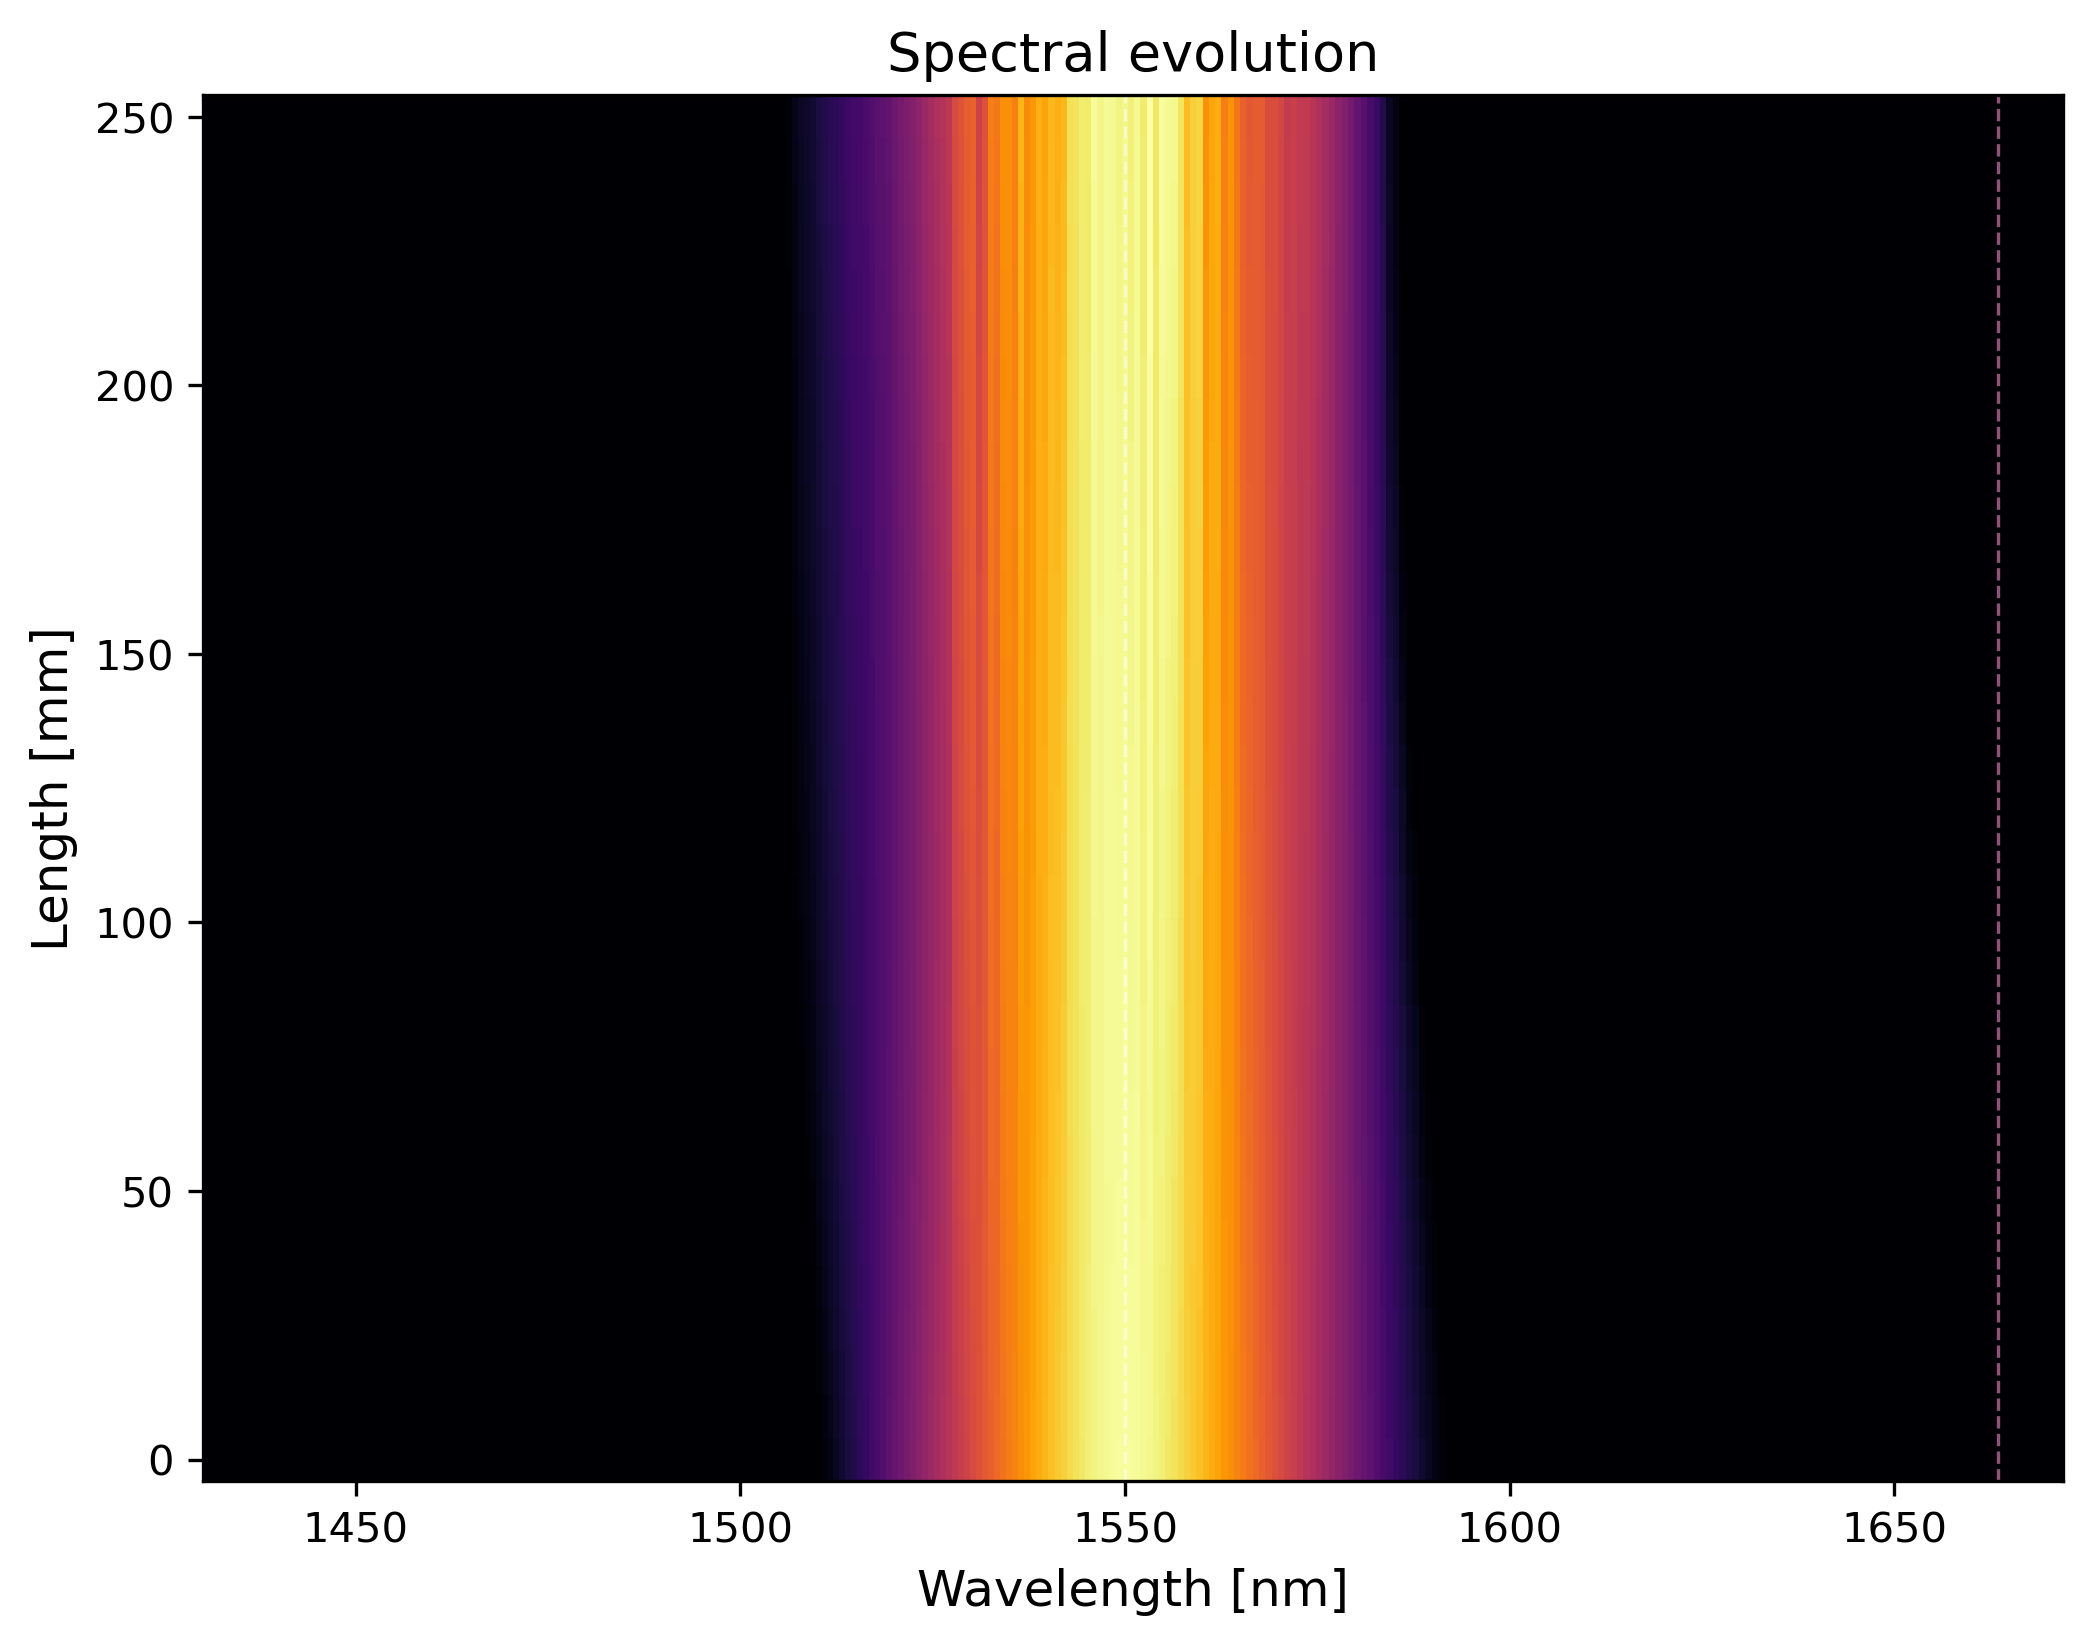
\includegraphics[height=0.31\textheight]{figures/reduced_trace_evolution.png}
\caption{Trace penalty on the reduced-control operating point. The best
reduced-control tolerance result reached about \(-66.44\,\mathrm{dB}\) with
\(\sigmathreedb\approx0.077\,\mathrm{rad}\). This confirms that the
robustness-depth tradeoff is not only a full-grid artifact.}
\end{figure}

\section{Key Numerical Results}

\begin{table}[H]
\centering
\small
\resizebox{\linewidth}{!}{%
\begin{tabular}{llllr}
\toprule
Operating point & Objective & Raman depth & \(\sigmathreedb\) & Geometry \\
\midrule
Full-grid & plain & \(-76.86\,\mathrm{dB}\) & \(0.025\,\mathrm{rad}\) & indefinite \\
Full-grid & MC, strongest tolerance & \(-73.01\,\mathrm{dB}\) & \(0.039\,\mathrm{rad}\) & indefinite \\
Full-grid & SAM, best tested & \(-78.38\,\mathrm{dB}\) & \(0.020\,\mathrm{rad}\) & indefinite \\
Full-grid & trace, strongest tolerance & \(-66.79\,\mathrm{dB}\) & \(0.083\,\mathrm{rad}\) & indefinite \\
Reduced-control & plain & \(-82.56\,\mathrm{dB}\) & \(0.011\,\mathrm{rad}\) & indefinite \\
Reduced-control & MC, strongest tolerance & \(-67.98\,\mathrm{dB}\) & \(0.077\,\mathrm{rad}\) & indefinite \\
Reduced-control & trace, strongest tolerance & \(-66.44\,\mathrm{dB}\) & \(0.077\,\mathrm{rad}\) & indefinite \\
\bottomrule
\end{tabular}}
\caption{Representative numerical results from the sharpness/robustness sweep.
The table keeps only the comparison points needed to interpret the tradeoff;
the full sweep contained \(26\) successful records.}
\end{table}

\section{Interpretation}

The first lesson is that robustness penalties do work in the limited sense that
they can increase \(\sigmathreedb\). The strongest full-grid trace case moved
from \(0.025\,\mathrm{rad}\) to \(0.083\,\mathrm{rad}\), and the strongest
reduced-control cases reached about \(0.077\,\mathrm{rad}\).

The second lesson is that the price is large. The strongest full-grid trace
case lost about \(10\,\mathrm{dB}\) of Raman depth. The reduced-control
high-tolerance cases lost even more depth relative to their very deep plain
reference. That is why the default objective should not be replaced.

The third lesson is that ``robust'' and ``convex-looking'' are different
claims. All resolved Hessian spectra remained indefinite. In other words, the
robustness penalties widened perturbation tolerance in some cases, but they did
not turn the local landscape into a simple bowl.

\subsection*{TLDR}

If I had to explain the result quickly: the sharpness lane found useful knobs,
not a new default. Trace regularization can make the phase less fragile, MC can
help a little more cheaply, SAM did not help much here, and the Hessian still
says the landscape is saddle-like.

\section{Presentation Capsule}

If this note becomes a robustness slide, the clean message is:
\begin{itemize}
    \item Deep suppression and robust suppression are different axes; the deepest mask can be experimentally fragile.
    \item Sharpness penalties intentionally trade some Raman depth for larger tolerance to phase perturbations.
    \item The most useful visual is the depth-versus-robustness tradeoff, not a short-fiber before/after image.
    \item The Hessian evidence still shows saddle-like geometry, so robustness penalties are knobs, not a proof that the landscape became simple.
\end{itemize}

\section{Limitations}

The robustness metric uses random phase perturbations, which are a useful proxy
for shaper error but not a complete model of an experimental pulse shaper.
Real hardware errors can have wavelength-dependent structure, calibration
offsets, amplitude coupling, finite resolution, and repeatability limits.

The Hessian diagnostics are finite-difference diagnostics around the final
solution. They are not a second-order optimizer, and the result depends on the
chosen scalar objective and control space. In particular, the reduced-control
Hessian should be read as curvature in coefficient space, not as a claim about
every full-grid direction.

The trace penalty uses a stochastic trace estimator with fixed probes. That is
the right deterministic choice for L-BFGS, but it still estimates only a
sampled curvature quantity. Increasing probe count or testing structured
hardware-like perturbations would be useful follow-up work.

\section{Reproduction Capsule}

The current sharpness research drivers live under
\texttt{scripts/research/sharpness/}. The expected workflow is:

\begin{enumerate}
    \item Run the batch driver with Julia threading enabled:
    \begin{center}
    \texttt{julia -{}-project=. -t auto scripts/research/sharpness/run.jl}
    \end{center}
    \item Summarize the completed sweep:
    \begin{center}
    \texttt{julia -{}-project=. -t auto scripts/research/sharpness/summarize.jl}
    \end{center}
    \item Inspect representative standard images before interpreting the
    results.
\end{enumerate}

Substantial reruns belong on the burst machine using the project heavy-job
wrapper. The important outputs are the completed record bundle, the
robustness-depth plot, the summary table, and the standard image sets for
representative plain, MC, SAM, and trace cases.

\section{Sources and References}

\begin{thebibliography}{9}
\bibitem{agrawal2019}
G. P. Agrawal. \textit{Nonlinear Fiber Optics}, 6th ed. Academic Press, 2019.
\url{https://www.sciencedirect.com/book/9780128170427/nonlinear-fiber-optics}

\bibitem{dudley2006}
J. M. Dudley, G. Genty, and S. Coen. ``Supercontinuum generation in photonic
crystal fiber.'' \textit{Reviews of Modern Physics}, 78, 1135--1184, 2006.
\url{https://doi.org/10.1103/RevModPhys.78.1135}

\bibitem{hult2007}
J. Hult. ``A fourth-order Runge-Kutta in the interaction picture method for
simulating supercontinuum generation in optical fibers.'' \textit{Journal of
Lightwave Technology}, 25(12), 3770--3775, 2007.
\url{https://doi.org/10.1109/JLT.2007.909373}

\bibitem{liu1989}
D. C. Liu and J. Nocedal. ``On the limited memory BFGS method for large scale
optimization.'' \textit{Mathematical Programming}, 45, 503--528, 1989.
\url{https://doi.org/10.1007/BF01589116}

\bibitem{nocedal2006}
J. Nocedal and S. J. Wright. \textit{Numerical Optimization}, 2nd ed.
Springer, 2006. \url{https://link.springer.com/book/10.1007/978-0-387-40065-5}

\bibitem{foret2021}
P. Foret, A. Kleiner, H. Mobahi, and B. Neyshabur. ``Sharpness-Aware
Minimization for Efficiently Improving Generalization.'' ICLR, 2021.
\url{https://arxiv.org/abs/2010.01412}

\bibitem{kwon2021}
J. Kwon, J. Kim, H. Park, and I. K. Choi. ``ASAM: Adaptive Sharpness-Aware
Minimization for Scale-Invariant Learning of Deep Neural Networks.'' ICML,
2021. \url{https://proceedings.mlr.press/v139/kwon21b.html}

\bibitem{zhuang2022}
J. Zhuang, B. Gong, L. Yuan, Y. Cui, H. Adam, N. Dvornek, J. Tatikonda,
J. Duncan, and T. Liu. ``Surrogate Gap Minimization Improves Sharpness-Aware
Training.'' ICLR, 2022. \url{https://arxiv.org/abs/2203.08065}

\bibitem{hutchinson1989}
M. F. Hutchinson. ``A stochastic estimator of the trace of the influence matrix
for Laplacian smoothing splines.'' \textit{Communications in Statistics -
Simulation and Computation}, 18(3), 1059--1076, 1989.
\url{https://doi.org/10.1080/03610918908812806}

\bibitem{meyer2021}
R. A. Meyer, C. Musco, C. Musco, and D. P. Woodruff. ``Hutch++: Optimal
Stochastic Trace Estimation.'' 2021. \url{https://arxiv.org/abs/2010.09649}

\bibitem{nohadani2007}
O. Nohadani, J. A. Desai, C. K. Fyfe, and D. Bertsimas. ``Robust Optimization
in Electromagnetic Scattering Problems.'' \textit{Journal of Applied Physics},
101, 074507, 2007. \url{https://doi.org/10.1063/1.2715540}
\end{thebibliography}

\end{document}
